%%
%% This is file `sample-acmsmall-conf.tex',
%% generated with the docstrip utility.
%%
%% The original source files were:
%%
%% samples.dtx  (with options: `acmsmall-conf')
%% 
%% IMPORTANT NOTICE:
%% 
%% For the copyright see the source file.
%% 
%% Any modified versions of this file must be renamed
%% with new filenames distinct from sample-acmsmall-conf.tex.
%% 
%% For distribution of the original source see the terms
%% for copying and modification in the file samples.dtx.
%% 
%% This generated file may be distributed as long as the
%% original source files, as listed above, are part of the
%% same distribution. (The sources need not necessarily be
%% in the same archive or directory.)
%%
%%
%% Commands for TeXCount
%TC:macro \cite [option:text,text]
%TC:macro \citep [option:text,text]
%TC:macro \citet [option:text,text]
%TC:envir table 0 1
%TC:envir table* 0 1
%TC:envir tabular [ignore] word
%TC:envir displaymath 0 word
%TC:envir math 0 word
%TC:envir comment 0 0
%%
%%
%% The first command in your LaTeX source must be the \documentclass
%% command.
%%
%% For submission and review of your manuscript please change the
%% command to \documentclass[manuscript, screen, review]{acmart}.
%%
%% When submitting camera ready or to TAPS, please change the command
%% to \documentclass[sigconf]{acmart} or whichever template is required
%% for your publication.
%%
%%
\documentclass[acmsmall]{acmart}

%%
%% \BibTeX command to typeset BibTeX logo in the docs
\AtBeginDocument{%
  \providecommand\BibTeX{{%
    Bib\TeX}}}

%% Rights management information.  This information is sent to you
%% when you complete the rights form.  These commands have SAMPLE
%% values in them; it is your responsibility as an author to replace
%% the commands and values with those provided to you when you
%% complete the rights form.
\setcopyright{acmcopyright}
\copyrightyear{2018}
\acmYear{2018}
\acmDOI{XXXXXXX.XXXXXXX}

%% These commands are for a PROCEEDINGS abstract or paper.
\acmConference[Conference acronym 'XX]{Make sure to enter the correct
  conference title from your rights confirmation emai}{June 03--05,
  2018}{Woodstock, NY}
%%
%%  Uncomment \acmBooktitle if the title of the proceedings is different
%%  from ``Proceedings of ...''!
%%
%%\acmBooktitle{Woodstock '18: ACM Symposium on Neural Gaze Detection,
%%  June 03--05, 2018, Woodstock, NY}
\acmPrice{15.00}
\acmISBN{978-1-4503-XXXX-X/18/06}


%%
%% Submission ID.
%% Use this when submitting an article to a sponsored event. You'll
%% receive a unique submission ID from the organizers
%% of the event, and this ID should be used as the parameter to this command.
%%\acmSubmissionID{123-A56-BU3}

%%
%% For managing citations, it is recommended to use bibliography
%% files in BibTeX format.
%%
%% You can then either use BibTeX with the ACM-Reference-Format style,
%% or BibLaTeX with the acmnumeric or acmauthoryear sytles, that include
%% support for advanced citation of software artefact from the
%% biblatex-software package, also separately available on CTAN.
%%
%% Look at the sample-*-biblatex.tex files for templates showcasing
%% the biblatex styles.
%%

%%
%% The majority of ACM publications use numbered citations and
%% references.  The command \citestyle{authoryear} switches to the
%% "author year" style.
%%
%% If you are preparing content for an event
%% sponsored by ACM SIGGRAPH, you must use the "author year" style of
%% citations and references.
%% Uncommenting
%% the next command will enable that style.
%%\citestyle{acmauthoryear}
\usepackage{booktabs}   %% For formal tables:
                        %% http://ctan.org/pkg/booktabs
\usepackage{subcaption} %% For complex figures with subfigures/subcaptions
                        %% http://ctan.org/pkg/subcaption

%%%%%%%%%%%%%%%%%%%%%%%%%%%%SELF DEFINED AND INPUTS%%%%%%%%%%%%%%%%%%%%%%%%%%%%%%%%%%%%%%%%%%

\usepackage[T1]{fontenc}
\usepackage[normalem]{ulem}
\usepackage{mathtools}
\usepackage{blkarray,bigstrut} 
\usepackage{graphicx,wrapfig,lipsum}
\usepackage{tcolorbox}
\usepackage{enumitem}
\usepackage{array}
\usepackage{algorithm}
\usepackage{algorithmic}
\usepackage{mathpartir}
\usepackage{multirow}
\usepackage{hyperref}
\usepackage{amssymb}
\usepackage{subcaption}
\usepackage{stmaryrd}
\usepackage{color} 


\usepackage{tikz}
\usetikzlibrary{snakes}
\usetikzlibrary{svg.path} 
\usetikzlibrary{calc} 
\usetikzlibrary{shapes}
\usetikzlibrary{shapes.geometric}
\usetikzlibrary{arrows.meta}
\usetikzlibrary{arrows}
\usetikzlibrary{decorations.text,decorations.markings}
% % % % 

%%%%%%%%%%Packages for adaoption%%%

% \usepackage{amsthm} 

%Packages

\input{ldefs}
\newcommand{\highlight}[1]{\textcolor[rgb]{.0,0.0,1.0}{ #1}}
\usetikzlibrary{shapes,arrows}
\newcommand{\THESYSTEM}{\textsf{PsRB}}

%%%%%%%%%%%%%%%%%%%%%%%%%%%%SELF DEFINED AND INPUTS%%%%%%%%%%%%%%%%%%%%%%%%%%%%%%%%%%%%%%%%%%

%%
%% end of the preamble, start of the body of the document source.
\begin{document}

%%
%% The "title" command has an optional parameter,
%% allowing the author to define a "short title" to be used in page headers.
\title[Short Title]{Path Sensitive Reachability Bound Analysis}         %% [Short Title] is optional;

%%
%% The "author" command and its associated commands are used to define
%% the authors and their affiliations.
%% Of note is the shared affiliation of the first two authors, and the
%% "authornote" and "authornotemark" commands
%% used to denote shared contribution to the research.
%% Author with single affiliation.
\author{First1 Last1}
\authornote{with author1 note}          %% \authornote is optional;
                                        %% can be repeated if necessary
\orcid{nnnn-nnnn-nnnn-nnnn}             %% \orcid is optional
\affiliation{
  \position{Position1}
  \department{Department1}              %% \department is recommended
  \institution{Institution1}            %% \institution is required
  \streetaddress{Street1 Address1}
  \city{City1}
  \state{State1}
  \postcode{Post-Code1}
  \country{Country1}                    %% \country is recommended
}
\email{first1.last1@inst1.edu}          %% \email is recommended

%% Author with two affiliations and emails.
\author{First2 Last2}
\authornote{with author2 note}          %% \authornote is optional;
                                        %% can be repeated if necessary
\orcid{nnnn-nnnn-nnnn-nnnn}             %% \orcid is optional
\affiliation{
  \position{Position2a}
  \department{Department2a}             %% \department is recommended
  \institution{Institution2a}           %% \institution is required
  \streetaddress{Street2a Address2a}
  \city{City2a}
  \state{State2a}
  \postcode{Post-Code2a}
  \country{Country2a}                   %% \country is recommended
}
\email{first2.last2@inst2a.com}         %% \email is recommended
\affiliation{
  \position{Position2b}
  \department{Department2b}             %% \department is recommended
  \institution{Institution2b}           %% \institution is required
  \streetaddress{Street3b Address2b}
  \city{City2b}
  \state{State2b}
  \postcode{Post-Code2b}
  \country{Country2b}                   %% \country is recommended
}
\email{first2.last2@inst2b.org}         %% \email is recommended

%%
%% The abstract is a short summary of the work to be presented in the
%% article.
\begin{abstract}
Goal: bound the number of visiting times for every program control location, i.e., Solve the 
\emph{Reachability-Bound Program}.
\\
Motivation: State-of-Art Techniques 
\\
in paper~\cite{Sumit2010rechability,sinn2017complexity} : path-insensitive 
\\
in paper~\cite{GulwaniJK09} : path-sensitive and precise for estimating loop bounds,
but over-approximate reachability times of control location as the loop bound.
\\
in paper~\cite{ZulegerGSV11} : able to identify different paths from multiple-path loop, but aims to solve bounds for loop and path. They over-approximate reachability times of control location with loop bound.
\\
Contributions: 
\\
1. Solve the 
\emph{Reachability-Bound Program} precisely /(improve accuracy),
in two challenging classes of programs: Programs with Path-Sensitive Loops, and Programs with Nested Loops 
\\
2. Improved efficiency by abstracting program using the Difference Constraint-base method in \cite{sinn2017complexity}.
\\
3. Efficient implementation and evaluation results.
\end{abstract}

%%
%% The code below is generated by the tool at http://dl.acm.org/ccs.cfm.
%% Please copy and paste the code instead of the example below.
%%
\begin{CCSXML}
<ccs2012>
 <concept>
  <concept_id>10010520.10010553.10010562</concept_id>
  <concept_desc>Computer systems organization~Embedded systems</concept_desc>
  <concept_significance>500</concept_significance>
 </concept>
 <concept>
  <concept_id>10010520.10010575.10010755</concept_id>
  <concept_desc>Computer systems organization~Redundancy</concept_desc>
  <concept_significance>300</concept_significance>
 </concept>
 <concept>
  <concept_id>10010520.10010553.10010554</concept_id>
  <concept_desc>Computer systems organization~Robotics</concept_desc>
  <concept_significance>100</concept_significance>
 </concept>
 <concept>
  <concept_id>10003033.10003083.10003095</concept_id>
  <concept_desc>Networks~Network reliability</concept_desc>
  <concept_significance>100</concept_significance>
 </concept>
</ccs2012>
\end{CCSXML}

\ccsdesc[500]{Computer systems organization~Embedded systems}
\ccsdesc[300]{Computer systems organization~Redundancy}
\ccsdesc{Computer systems organization~Robotics}
\ccsdesc[100]{Networks~Network reliability}

%%
%% Keywords. The author(s) should pick words that accurately describe
%% the work being presented. Separate the keywords with commas.
\keywords{Loop Bound Inference, program refinement, path-sensitive}  %% \keywords are mandatory in final camera-ready submission


%% A "teaser" image appears between the author and affiliation
%% information and the body of the document, and typically spans the
%% page.
% \begin{teaserfigure}
%   \includegraphics[width=\textwidth]{adapfun}
%   \caption{Seattle Mariners at Spring Training, 2010.}
%   \Description{Enjoying the baseball game from the third-base
%   seats. Ichiro Suzuki preparing to bat.}
%   \label{fig:teaser}
% \end{teaserfigure}

\received{20 February 2007}
\received[revised]{12 March 2009}
\received[accepted]{5 June 2009}

%%
%% This command processes the author and affiliation and title
%% information and builds the first part of the formatted document.
\maketitle


\section{Introduction}
\label{sec:intro}

Gulwani et. al~\cite{GulwaniZ10} first introduce \emph{reachability-bound} as the upper bound on the number of times a given control location 
inside a procedure is visited during program execution.
A tight reachability-bound has many applications.
For example from a privacy and security perspective,
how much secret information is leaked by a program depends on the number of times a certain operation that leaks the data
is executed~\cite{Malacaria07};
from an efficiency perspective, when different program locations consume different resources, a precise reachability-bound of each location can help to estimate the resource cost more accurate than just computing the overall complexity.
While existing works all have different limitations when inferring the \emph{reachability-bound}.
For example, Gulwani et. al~\cite{GulwaniZ10}
give a two-step solution by combining program abstract and proof-rules-based bound computation.
But it does not compute the \emph{reachability-bound} precisely for every control location.
Instead, they only compute the complexity bounds for overall loop and over-approximate for different locations using this bound,
which is loose especially when there are multipath loops.
Techniques in program complexity analysis~\cite{GustafssonEL05,HumenbergerJK18} 
or worst-case resource cost analysis
~\cite{BrockschmidtEFFG16,AlbertAGP08,AliasDFG10,Flores-MontoyaH14} can be repurposed to estimate similar quantities such as the
bounds on loop iterations, execution time, etc.
While these quantities focus only on  
the overall complexity,
none of them compute the reachability-bound on a given program control location directly or path-sensitively.
This leads to inaccuracy in data leakage analysis, resource cost estimation, etc.
To overcome these limitations, 
we introduce a novel path-sensitive reachability-bound analysis algorithm that solve 
the reachability-bounds problem efficiently and path-sensitively.
It is built over an abstract transition graph which effectively combines amortized complexity analysis with loop summarization based multipath refinement.
This combination mitigates the limitations faced by either technique individually. 
Before diving into the algorithm, below are some related works and their limitations.

% \begin{itemize}
% \item 
\emph{Program Abstraction.}
Program abstraction is commonly used in program analysis as a preprocessing step to abstract program features and generate transition graphs or systems. For example, Gulwani et. al~\cite{GulwaniZ10} summarizes programs into some underlying abstract domains (the unified lattice~\cite{CousotH78}, polyhedra~\cite{CousotC77} or octagonal~\cite{Mine06})
and generates transition systems for loop counters.
\cite{KincaidCBR18} abstracts program into the wedge domain and computes the non-linear loop invariant.
%  While it only works well for the specific targeting problem.
Efficiency is the main bottleneck when generating and solving the constraint.
We choose to use the difference constraint based program abstraction model~\cite{SinnZV17,SinnZV14} combined with boolean expression to generate our abstract transition graph.
It is more accurate in the sense of representing the program loops path-sensitively. This representation is also comparatively lightweight.

% \item 
\emph{Amortized Complexity Analysis.}
One line of complexity analysis follows the idea of the \emph{amortized complexity analysis}
originated from Tarjan's influential paper~\cite{PotechinP17}. It is usually combined with ranking functions~\cite{BradleyMS05,CookSZ13,Zuleger18} or counter increments~\cite{ZulegerGSV11,SinnZV14,SinnZV17,LuCT21,AliasDFG10}.
They do well in nested loops by alternating the loop bound computation with the ranking or counter estimation. This alternation is efficient without recursively unrolling the nested loops when composing the bound of different paths.
  % \\
  But estimating the counter or ranking function invariant ignores the interleaving between multiple paths in the same loop,
% Most of them 
such as the tools CofloCo~\cite{Montoya17,Flores-MontoyaH14,Flores-Montoya16}, KoAT~\cite{BrockschmidtEFFG16,BrockschmidtEFFG14,FalkeKS12,FalkeKS11}, the algorithm in~\cite{LuCT21}, and etc.
%  over-approximate the loop bound when the path interleaving affects loop execution.
It is hard to repurpose their result as the reachability-bound on different points.
% loop bound path-insensitively as the reachability-bound on different points.
Another kind of \emph{amortized complexity analysis} based on type refinement or annotation~\cite{CraryW00,JostHLH10,CicekBG0H17,RajaniG0021,CarbonneauxHS15} has the same weakness in the multipath loops, resulting in the over-approximation of the resource cost on different program points.
To overcome these limitations, we enrich it with path-sensitivity according to the Alg.~2 in~\cite{SinnZV14},
% which assigns a variable to each edge on which this variable decrease as its ranking function.
the Alg.~3 in~\cite{ZulegerGSV11},
and the Def.~25 in Section 4 from~\cite{SinnZV17}.

\emph{Loop Summarization and Path Refinement Based Complexity Analysis}.
Another line of loop bound analysis through loop summarization and path refinement seeks for precise loop path representation~\cite{ManoliosV06,BalakrishnanSIG09,SharmaDDA11,Flores-MontoyaH14,HumenbergerJK18,CyphertBKR19}, and explicating the interleaving between paths~\cite{GulwaniJK09,ZulegerGSV11}.
\cite{KincaidBCR19,KincaidCBR18,BreckCKR20} introduce some loop summarization techniques which can help to improve the accuracy of the path refinement but specifically for non-linear loops, program recurrence, etc.
%  summarization techniques~\cite{KincaidCBR18} and the invariant generating algorithm considering recurrence in~\cite{BreckCKR20}. 
However, when composing the bound between nested loops, recursively unrolling the nested loops is heavy and non-terminating in most cases.
%
Our method simplifies the path refinement algorithm in~\cite{GulwaniJK09} using contextualization techniques based on~\cite{ZulegerGSV11,SinnZV14,ManoliosV06}.
We also limit the iterations of the refinement algorithm to a constant in our bound analysis algorithm.
% \end{itemize}
%

We perform both path refinement and ranking estimation over an abstract transition graph through program abstraction presented in Section~\ref{sec:progabs}.
This combination utilizes the effectiveness of \emph{amortized complexity analysis} by computing the ranking function
% $\locbound(\absevent, c)$ for each transition edge $\absevent$, 
and estimating its bound invariant in Section~\ref{sec:rank}.
It additionally benefits from the accuracy of path refinement techniques through a light-weight path refinement algorithm adopted from~\cite{GulwaniJK09} in Section~\ref{sec:refine}.
Building on this combination, we introduce two novel quantities,
the \emph{path reachability-bound} and \emph{loop reachability-bound}.
The first one bounds the evaluation times of each loop free and interleaving free path in a refined program, and the second one bounds the iterations of an outer loop w.r.t. the innermost loop such that in these iterations of outer loop, the innermost loop is ``entered''. 
Then we present the algorithm for estimating the two quantities in Section~\ref{sec:looprb} and~\ref{sec:pathrb} and compute the \emph{reachability-bound} for each program point path-sensitively in Section~\ref{sec:psrb}.
Our evaluation on the prototype implementation in Section~\ref{sec:eval} shows that we can accurately estimate different bounds for different program points on multiple loop paths. By summing up the different \emph{reachability-bound}s on every location, the results shows a big improvement comparing to the state-of-art worst case complexity analysis.

To recapitulate, our main contributions are summarized as follows.
\\
% \begin{itemize}
%   \item 
1. A path-sensitive reachability-bound algorithm which computes sound bound on the evaluation times of each program point path-sensitively.
\\
%  \item 
2. The combination of \emph{amortized bound analysis} through ranking function estimation and the path refinement approach in our algorithm.
% \item 
\\
3. Two novel quantities, the \emph{path reachability-bound} and \emph{loop reachability-bound} and their corresponding estimating algorithms.
% \item 
\\
4. A prototype implementation with evaluation over four different benchmarks.
  The evaluation shows big improvement comparing to the state-of-art worst case complexity analysis, and potential applications in other areas.
% \end{itemize}
\section{Overview}
\label{sec:overview}
In this section, we discuss a representative running examples with
challenges of analyzing the symbolic
\emph{reachability-bound} on
every control location and illustrate our key novelties, \emph{path reachability-bound} and the \emph{loop reachability-bound}.
This example is adopted from the example in~\cite{GulwaniZ10}, which
is a skeleton code from the .Net base-class library.

% \paragraph{Challenges.}
\begin{example}
  [The Running Example with Two Paths Loop and Nested Loop in One Path]
  \label{ex:relatedNestedWhileOdd_abscfg}
    { \small
  \begin{figure}
  \centering
  \begin{subfigure}{.4\textwidth}
    \begin{centering}
    {\small
    $
    \begin{array}{l}
      \kw{nestedOdd}(n, m) \triangleq \\
      \clabel{ \assign{i}{n} }^{0} ; \\
          \ewhile ~ \clabel{i > 0}^{1} ~ \edo ~ \\
          \qquad \Big(
            \eif(\clabel{i \% 2 \neq 0 }^{2},\\
            \qquad \clabel{\assign{k}{i - m}}^{3};\\
            \qquad \ewhile ~ \clabel{k > 0}^{4} ~ \edo ~
            \Big( \clabel{\assign{k}{k - 1}}^{5} \Big);\\
            \qquad \clabel{\assign{i}{k + m}}^{6};
            \clabel{\assign{i}{i - 1}}^{7}, \\
            \qquad \clabel{\assign{i}{i - 3}}^{8})
            \Big)
      \end{array}
    $
    }
    \caption{}
    \end{centering}
    \end{subfigure}
  \begin{subfigure}{.5\textwidth}
    \begin{centering}
  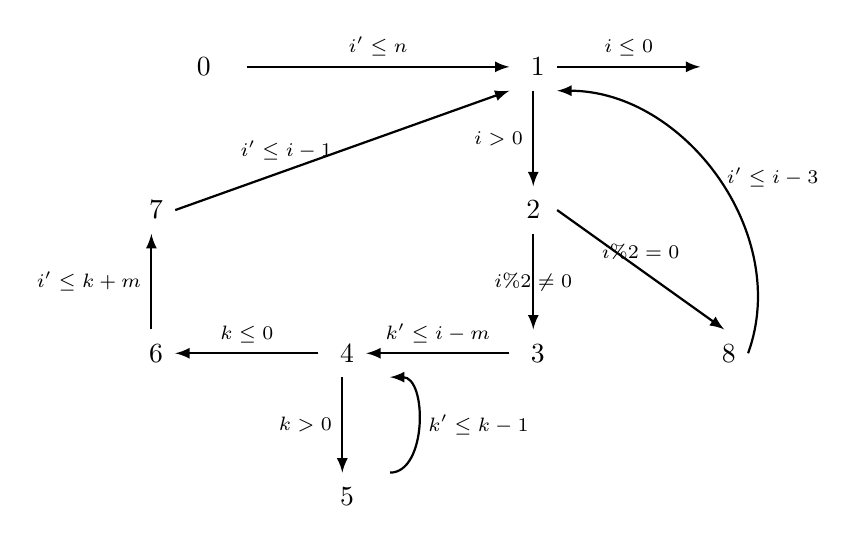
\begin{tikzpicture}[scale=\textwidth/20cm,samples=200]
  \draw[] (-7, 10) circle (0pt) node{{ $0$}};
  \draw[] (0, 10) circle (0pt) node{{ $1$}};
  \draw[] (0, 7) circle (0pt) node{\textbf{$2$}};
  \draw[] (0, 4) circle (0pt) node{{ $3$}};
  \draw[] (-4, 4) circle (0pt) node{{ $4$}};
  \draw[] (-8, 4) circle (0pt) node{{ $6$}};
  \draw[] (-4, 1) circle (0pt) node{{ $5$}};
  \draw[] (4, 4) circle (0pt) node{{ $8$}};
  \draw[] (-8, 7) circle (0pt) node{{ $7$}};
  % Counter Variables
  \draw[] (4.5, 10) circle (0pt) node {\textbf{$\lex$}};
  % \draw[] (6, 4) circle (0pt) node {{ $ex$}};
  %
  % Control Flow Edges:
  \draw[ thick, -latex] (-6, 10)    -- node [above] {\scriptsize $i' \leq n$}(-0.5, 10);
  \draw[ thick, -latex] (0, 9.5)    -- node [left] {\scriptsize $i > 0$} (0, 7.5) ;
  \draw[ thick, -latex] (0.5, 7)    -- node [above] {\scriptsize $ i \% 2 = 0 $}  (4, 4.5);
  \draw[ thick, -latex] (4.5, 4)    to  [out=70,in=0]   node [right] {\scriptsize $i' \leq i - 3$ }(0.5, 9.5);
  \draw[ thick, -latex]  (0, 6.5)   -- node  {\scriptsize $i \% 2 \neq 0$}  (0, 4.5) ;
  \draw[ thick, -latex]  (-0.5, 4)  -- node [above] {\scriptsize $k' \leq i - m$ }  (-3.5, 4) ;
  \draw[ thick, -latex]  (-4.5, 4)  -- node [above] {\scriptsize $k \leq 0$ }  (-7.5, 4);
  \draw[ thick, -latex] (0.5, 10)   -- node [above] {\scriptsize $i \leq 0$}  (3.5, 10);
  \draw[ thick, -latex] (-4, 3.5)   -- node [left] {\scriptsize $k > 0$}  (-4, 1.5);
  \draw[ thick, -latex] (-3, 1.5)   to  [out=0,in=0] node [right] {\scriptsize $k' \leq k- 1$}  (-3, 3.5);
  \draw[ thick, -latex] (-8, 4.5)   --  node [left] {\scriptsize $i' \leq k + m$ }(-8, 6.5);
  \draw[ thick, -latex] (-7.5, 7)  --  node [left] {\scriptsize $i' \leq i - 1$ }(-0.5, 9.5);
  % \draw[ thick, -latex] (6, 6.5)  -- node [right] {$\top$} (6, 4.5) ;
  \end{tikzpicture}
  \caption{}
    \end{centering}
    \end{subfigure}
\begin{subfigure}{.9\textwidth}    
\begin{centering}
  {\small
  $\tpath_0 = (0 \to 1)$
  \quad
  $\tpath_1 = (1 \to 2 \to 3 \to 4)$
  \quad
  $\tpath_2 = (4 \to 6 \to 7 \to 1)$
  \quad
  $\tpath_3 = (4 \to 5 \to 4)$
  \quad
  $\tpath_4 = (1 \to 2 \to 8 \to 1)$
  \quad
  $\tpath_5 = (1 \to \lex)$
  \\
  $
  \tpath_0 ; \rpchoose{ 1: \rprepeat(\tpath_1; 4:\rprepeat(\tpath_3); \tpath_2; \tpath_4), 
  1: \rprepeat(\tpath_4; \tpath_1; 4:\rprepeat(\tpath_3); \tpath_2) }; \tpath_5
  $
  }
  % \caption{}
    \end{centering}
    \end{subfigure}
  \caption{
  (a) The program of the two paths loop with a nested Loop in one path,
    (b) The corresponding \emph{Abstract Transition Graph}, $\absG(\kw{nestedOdd}(n, m))$. }
      \label{fig:relatedNestedWhileOdd-overview}
  \end{figure}
  }
  %
  \end{example}    
  
\footnotetext{We use the notation $(l_0 \to \cdots \to l_n)$ to denote a vertices sequence $(l_0, \cdots, l_n)$, and the constraint on each edge in each transition path are omitted for concise.}
% \todo{Shorten}
% \begin{itemize}
%   \item 
\textbf{Challenge I}
  In this example, given $n \geq m$,
the precise \emph{reachability-bound}s for control locations $4$ and $5$ are both $m \times \lfloor\frac{n}{m}\rfloor$,
for location $2$ and $3$ are $(m + 1) \times \lfloor\frac{n}{m}\rfloor + 1$, 
and $1$ for locations $0, 1$ and $\lex$. 
\highlight{Notice here, though within the same loop $L_2$, the bounds for locations $4$ and $5$ on the first branch, and $6$ on the second branch are different.}
\\
However, the state-of-art \emph{reachability-bound} analysis~\cite{GulwaniZ10}
gives the same \emph{reachability-bound}, $n + \lfloor\frac{n}{m}\rfloor$ for all the locations within the loop $L_2$, which is tight w.r.t. $L_2$'s iteration times but not for different locations inside $L_2$ without considering multiple paths.
Among works on program complexity, cost and loop bound analysis, \cite{GulwaniJK09} can also compute the tight bound on the loop iteration but not reachability-bound on each location path-sensitively.
Though we can use it as the \emph{reachability-bound} for location $1$ and $2$,
the \emph{reachability-bounds} for control locations $4, 5$ and $6$ are still unclear.

This motivates us the first key novelty -- the \emph{path reachability-bound} $\inoutB(\rprog, \tpath)$ for a loop free path $\tpath$ within a loop program $\rprog$ bounds the evaluation times of each loop free path instead of the entire multipath loop.
% \item 

\textbf{Challenge II}
  Then in line 8, $i$ is reset by $w$ and $w$ is reset by $j$ at line 5. So the
while $L_6$ is only executed in the first iteration of while loop $L_1$ and $L_3$.
% \\
The while loop $L_3$ at line 3 is executed only in 
the first $m - N$ iterations of the 
$L_1$ because $j$ is reset by $i$ in line 2.
% \\
So the total iterations of all the three loops is
$n + m^2 - m \times N$,
and the precise \emph{reachability-bound} for location $7$ inside the $L_6$ is $N$,
for locations $4, 5$ and $8$ between the $L_3$ and $L_6$ are $(n-N) \times (m - N)$,
and $n - N$ for locations $2$ and $9$.
% \\
\highlight{Notice here the \emph{reachability-bounds} for the locations inside the loop $L_6$ is 
the same as its innermost loop iteration bound.
% , as well as our \emph{path reachability-bound}.
However, for the locations between $L_3$ and $L_6$,
the \emph{reachability-bounds} are the multiplication of the inner and outer loop iteration bounds.}
\\
To the best of our knowledge, the loop bound analysis method in \cite{GulwaniJK09} can only give a loose bound $n + (m \times n) + N$ for the entire loop complexity, and 
the DC-based algorithm in \cite{SinnZV17} is able to
compute a better but still loose bound, $n + m^2 - m \times N$ on total iteration times.
None of them can give the precise \emph{reachability-bound} for every location in these nested loops,
which is non-trivial to compute even though knowing the loop bound.
% especially for the locations similar to $7$ in $\kw{threeNestedWhile}$.

\highlight{
This motivates use consider our second novel quantity --
the numbers of iterations of the outside loop $L_3$ and $L_1$ such that,
during these iterations, the loop $L_6$ is ``entered''. 
We call this the \emph{loop reachability} of the location within loop $L_6$ w.r.t the loops $L_3$ and $L_1$.
Then by multiplying the loop iteration bound of the $L_6$ with its \emph{loop reachability} times w.r.t the  $L_3$ and $L_1$, we can compute the precise
\emph{reachability-bounds} for location $7$.
}

\highlight{
This quantity isn't considered or computed in any of the previous works.
In the line of methods based on path refinement and loop summarization, the \emph{Progress Invariant} method in \cite{GulwaniJK09} is only able to compute
the
bound on iteration numbers
of the inner loop $L_6$ in each iteration of $L_3$ and $L_1$, which are both $N$.
So they have to over-approximate the reachability-bound for locations inside $L_6$ with the
overall program complexity by multiplication, i.e., $n + m^2 - m \times N$.
In the line of the \emph{amortized complexity analysis} through ranking function, the DC-based algorithm in \cite{SinnZV17}
is only able to
compute the combined loop bound and the local bound of each loop
separately as well.
% We are still unable to know the precise \emph{reachability-bound} for the locations in the innermost loop.
}
% \end{itemize}
With the two key novelties, our algorithm computes the reachability-bound for this example through the following steps.
% \paragraph{Main Steps of Path-sensitive Reachability-bound Analysis}
% \label{sec:static_rb}

\textbf{\emph{Step1: Program abstraction.}}
In Section~\ref{sec:progabs},
we first 
generate the \emph{Abstract Transition Graph} as in Figure~\ref{fig:relatedNestedWhileOdd-overview}(b).
Each edge $l \xrightarrow{dc} l'$ is an abstract transition $\absevent = (l, dc, l')$ annotated with a constraint $dc$ corresponding to the command of label $l$.

Then we abstract the program in the form of paths.
$$
\tpath_0 ; \rpchoose{ 1: \rprepeat(\tpath_1; 4:\rprepeat(\tpath_3); \tpath_2), 1:\rprepeat(\tpath_4) }; \tpath_5
$$
$;$ concatenates sequence of execution paths,
$\rprepeat(\tpath_3)$ represents looping on the path $\tpath_3$ and
$\rpchoose{ \ldots}$ represents the loop $L_1$ which contains two possible execution paths,
$\rprog_1 = \tpath_1; 4:\rprepeat(\tpath_3);\tpath_2$ and $\rprog_2 =\tpath_4$.

% \textbf{Step 2: Program Refinement}
\textbf{\emph{Step 2: Path interleaving refinement.}} 
Two execution paths are not simply iterating on themselves during the program execution,
they could interleave each other at certain iteration.
We summarize each execution path into conjunctions of transition relations.
\begin{equation}
    \begin{array}{l}
        \rprog_1 \models \phi_1 = \\
    \rprog_2 \models \phi_2 = 
    \end{array}
\end{equation}
  
In this sense, Algorithm~\ref{alg:prog-refine} in Section~\ref{sec:refine} computes the interleaving orders
by exhaustively checking the compositions of transition relations of different execution paths,
\begin{equation}
    \begin{array}{l}
        \rprog_1 ; \rprog_1 \models \exists i, k \st \phi_1 \circ \phi_1 = ... \implies \efalse\\
        \rprog_2 ; \rprog_2 \models \exists i, k \st \phi_2 \circ \phi_2 = ... \implies \efalse \\
        \rprog_2 ; \rprog_1 \models \exists i, k \st \phi_2 \circ \phi_1 = ...  \\
        \rprog_1 ; \rprog_2 \models \exists i, k \st \phi_1 \circ \phi_2 = ... 
    \end{array}
\end{equation}
Only two execution paths are feasible, so we identify two unique interleaving orders --
either $\rprog_1$ executes after one iteration of $\rprog_2$ or vice versa.
% Then, loop $L_1$ in the source program is generates new execution paths as follows,
\[
    \rprog^1 = \rprog_1 ; \rprog_2 = \tpath_1; 4:\rprepeat(\tpath_3); \tpath_2; \tpath_4
    \qquad
    \rprog^2 = \rprog_2 ; \rprog_1 = \tpath_4; \tpath_1; 4:\rprepeat(\tpath_3); \tpath_2
\]
% The second step in Section~\ref{sec:refine}
Then, the multiple-paths loop $L_1$ in the source program is refined
into multiple loops where each one can only iterate following the specified interleaving order.
% the interleaving of paths is explicit.
As in the bottom of Figure~\ref{fig:relatedNestedWhileOdd-overview}(c),
the program is transformed into 
\[
    \tpath_0 ; \rpchoose{ 1: \rprepeat(\tpath_1; 4:\rprepeat(\tpath_3); \tpath_2; \tpath_4), 
1: \rprepeat(\tpath_4; \tpath_1; 4:\rprepeat(\tpath_3); \tpath_2) }; \tpath_5
\]
In this refined program, 
each new execution path is equivalent to the execution of the original loop. 
% denoted as $\rprog_1^1$ and $\rprog_1^2$.

% \textbf{Step 3: Ranking Function Estimation}
\textbf{\emph{Step 3: ranking function estimation.}}
Algorithms in Section~\ref{sec:rank} identifies the ranking function for each transition edge, which is a symbol whose number of decreasing times can represent the number of execution of this edge.
For example for edge $4 \to 5$, its ranking function is $k$ and edges on $\tpath_1$, $\tpath_2$ and $\tpath_4$ all have $i$ as their ranking functions.

% \textbf{Step 4: Path-sensitive Reachability-bound Computation.}
\textbf{\emph{Step 4: local path reachability-bound.}}
For $\tpath_3$ in the program in Figure~\ref{fig:relatedNestedWhileOdd-overview}, we want to know how many times it is ``reached'' during the program execution.
From the refined program, $\tpath_3$ shows up in both newly generated execution paths $\rprog^1$ and $\rprog^2$  and nested in two level loops.
The algorithm in Section~\ref{sec:pathlocalrb} first
% computes a local \emph{path reachability-bound} for it w.r.t. its innermost loop $L_4$ by computing 
computes three abstract states for the ranking functions on $\tpath_3$ when first, second and last visiting during execution of $L_4$,
\begin{equation*}
    \rfinit(\rprog^1, \tpath_3, c) = \{k = n - m\} \quad
    \rfnext(\rprog^1, \tpath_3, c) = \{k = 1\} \quad
    \rffinal(\tpath_3, c) = \{ k = 0 \}.
\end{equation*}
Then  the maximal value of the following formula provides   
an upper bound on the number of execution times of $\tpath_3$ when executing only the innermost loop where $\tpath_3$ is nested. 
\[
    \max
    \left\{ 
        {\frac{a - b}{1}} 
        ~\vert~
        x = a \in \{k = n - m\}
        \land x = b \in \{ k = 0 \}
    \right\}  = n - m
\]
% The algorithm in Section~\ref{sec:pathlocalrb}
% computes $\outinB(4:\rprepeat(\tpath_3), \tpath_3, c) = n - m$ by computing
% the initial state, next state and final state of ranking functions on $\tpath_3$ during the execution of $\rprepeat(\tpath_3)$.

\textbf{\emph{Step 5: loop reachability-bound.}}
Previous step only provides the path reachability-bound for a simple transition path w.r.t. the innermost loop.
For nested loops, we need to compute the \emph{loop reachability-bound} for each simple transition path with respect to every level of the outer loop.
Since $\tpath_3$ is nested in two level loops, we compute its \emph{loop reachability-bound}
with respect to the outer loop $L_1$. 
It is expected to be $1$ because the inner loop $L_4$ is reached only in the first iteration of the outer loop $L_1$.
% , we aim to compute $1$ as the \emph{loop reachability-bound} of $\tpath_3$ w.r.t. $L_1$.
In the first refined execution path, $\rprog^1 = \rprepeat(\tpath_1; 4:\rprepeat(\tpath_3); \tpath_2; \tpath_4)$,
we compute three abstract states when visiting $L_4$ the first, second and last time during the execution of loop $\rprog^1$,
\begin{equation*}
\lpinit(\rprog^1, \tpath_3, c) = \max\{ n - m\} \quad
\lpnext(\rprog^1, \tpath_3, c) = \max\{n - m\} \quad
\rffinal(\tpath_3, c) = \{k = 0\}.
\end{equation*}
Then we compute \emph{loop reachability-bound} as the maximal value of the formula,
\[
    \max\limits_{x = a \in \{k = 0\}}
    \frac{\lpinit(\max\{n - m\} - a }{\max\{n - m\}} = 1
  \]
We also compute in the second refined execution path $\rprog_1^2$ the same number.
% $\outinB(4:\rprepeat(\tpath_3), \tpath, c) = n - m - 3$ and the same $\lpchB(\rprog_1^2, \tpath_3, c)$.
% So 

\textbf{\emph{Step 6: path reachability-bound.}}
For each simple transition path in every refined execution path where it shows up, we take the production of the \emph{loop reachability-bound}
and local \emph{path reachability-bound}.
For example for $\tpath_3$ in the first refined execution path 
$\rprepeat(\tpath_1; 4:\rprepeat(\tpath_3); \tpath_2; \tpath_4)$,
we compute $1 \times (n - m)$ and $1 \times (n - m - 3)$ in the second execution path.
Then we
take the maximal value over all refined execution order and
$\inoutB(\rprog, \tpath_3, c) = \max\{ 1 \times (n - m), 1 \times (n - m - 3) \} = n - m$.
This maximization operation does not produce over-approximation because there does not exist interleave
between the refined execution paths and each refined execution path is equivalent to the original loop, and each other as well.

\textbf{\emph{Step 7: reachability-bound.}}
Now for every program point $l$, we sum up the $\inoutB(\rprog, \tpath)$ over all $\tpath$ that contains $l$ and get $\psRB(l, c)$.
Since point $5$ only shows up on $\tpath_3$, we compute \highlight{$\psRB(5, c) = n - m$}.
The points $0$ and $\lex$ are not in any loop, so we have $\psRB(0, c) = \psRB(\lex, c) = 1$.
The points $3, 6, 7$ and $8$ which only show up once on $\tpath_2$ and $\tpath_4$ are all equal to $\lfloor\frac{m}{4}\rfloor$ the same as their $\inoutB$.
For the loop headers $1$ and $4$, we only count the $\tpath$ where they show up as a start-point.
So $\psRB(4, c) = \lfloor\frac{m}{4}\rfloor + n - m + 1$ and $\psRB(1,c) = 2 \times \lfloor\frac{m}{4}\rfloor + 1$ all as expected.


% % The second key idea combining two lines of works above is the \emph{loop reachability-bound}, $\lpchB(L:\rprog, \tpath)$.
% % For each transition path $\tpath$ w.r.t each of the loops $L:\rprog$ in which $\tpath$ is nested,
% % $\lpchB(L:\rprog, \tpath)$ bounds the iterations for
% % the outside loop, $L:\rprog$ w.r.t. the innermost loop where $\tpath$ is enclosed,
% % such that during these iterations of $L:\rprog$, the innermost loop is ``entered''. 
% % Then by multiplication and summing over these two bounds where each program control point shows up, we compute each point's the \emph{reachability-bound} path-sensitively.

% \paragraph{The path reachability-bound}, $\inoutB(\rprog, \tpath)$ is our first key novelty.
% It is a bound for a loop free path $\tpath$ within a loop program $\rprog$ bounds the evaluation times of each loop free path instead of the entire multipath loop.
% \input{examples/whileTwoCounters-overview}
% \footnotetext{We use the notation $(l_0 \to \cdots \to l_n)$ to denote a vertices sequence $(l_0, \cdots, l_n)$, and the constraint on each edge in each transition path are omitted for concise.}
% Figure~\ref{fig:whileTwoCounters-overview}(a) shows an example of a two paths loops
% with different \emph{reachability-bounds} on the control locations in different paths.
% This example is adopted from the example in~\cite{GulwaniZ10}, which
% is a skeleton code from the .Net base-class library.
% \\
% In this example, given $n \geq m$,
% the precise \emph{reachability-bound}s for control locations $4$ and $5$ are both $m \times \lfloor\frac{n}{m}\rfloor$,
% for location $2$ and $3$ are $(m + 1) \times \lfloor\frac{n}{m}\rfloor + 1$, 
% and $1$ for locations $0, 1$ and $\lex$. 
% \highlight{Notice here, though within the same loop $L_2$, the bounds for locations $4$ and $5$ on the first branch, and $6$ on the second branch are different.}
% \\
% However, the state-of-art \emph{reachability-bound} analysis~\cite{GulwaniZ10}
% gives the same \emph{reachability-bound}, $n + \lfloor\frac{n}{m}\rfloor$ for all the locations within the loop $L_2$, which is tight w.r.t. $L_2$'s iteration times but not for different locations inside $L_2$ without considering multiple paths.
% Among works on program complexity, cost and loop bound analysis, \cite{GulwaniJK09} can also compute the tight bound on the loop iteration but not reachability-bound on each location path-sensitively.
% Though we can use it as the \emph{reachability-bound} for location $1$ and $2$,
% the \emph{reachability-bounds} for control locations $4, 5$ and $6$ are still unclear.

% To compute the bounds for locations on different paths of a loop, we compute the \emph{path reachability-bound},
% which is the first key idea of this path-sensitive \emph{reachability-bound} analysis algorithm. This bound approximate the evaluation times of each loop free path instead of the entire multipath loop.
% \\
% This bound is computed based on the refined loop and using the estimated ranking function for every path, combines two lines of work introduced in Section~\ref{sec:intro}. It is benefited from the high accuracy of the path refinement and the ranking function estimation, but reduces the efficiency comparing to simply computing the ranking function.
% \\
% % Our algorithm combines the idea of \emph{difference constraint} based program complexity analysis method from \cite{SinnZV17}
% % and the control-flow refinement technique from~\cite{GulwaniJK09}.
% For this example, we first
% generate the abstract transition graph for the program using the difference constraints, such as Figure~\ref{fig:whileTwoCounters-overview}(b).
% Then it transforms every loop in $\kw{twoPathsWhile}$ by explicitly computing the interleaving between paths and
% %  using the control-flow refinement technique from~\cite{GulwaniJK09} and 
% generates a refined program $\rprog$ as
% \\
% % 
% % The refined program for program $\kw{twoPathsWhile}$ is
% % \[
%   $
%   \tpath_0 ; 
%   \rpchoose{2: \rprepeat_2(\rprepeat_1(\tpath_1); \tpath_2), 
%   2: \rprepeat_1(\tpath_1)}; \tpath_3.
%   $
% % \]
% \\
% Each $\tpath_i$ in this refined program is a \emph{simple transition path} we computed in a pre-procedure, which is loop free and not interleave with the other $\tpath_j, j \neq i$ as in Figure~\ref{fig:whileTwoCounters-overview}(c).
% % Every path will not interleave with the others. 
% Then we compute the \emph{path reachability-bound} for every $\tpath_i$,
% $\inoutB(\rprog, \tpath_i)$ during the execution of $\rprog$.
% % which is a bound on the reachability time of $\tpath$ during the execution of $\rprog$.
% The \emph{path reachability-bound}s for the four simple transition paths in this example are
% $\inoutB(\rprog, \tpath_1) = \max\{m, m \times \lfloor\frac{n}{m}\rfloor\}$,
% $\inoutB(\rprog, \tpath_2) = \lfloor\frac{n}{m}\rfloor$,
% and $\inoutB(\rprog, \tpath_0) = \inoutB(\rprog, \tpath_3) = 1$.
% % \\
% % Then we use this bounds
% % and another \emph{loop reachability-bound}
% % to compute the final \emph{reachability-bound} for each location.
% Since there isn't nested loop in this example, we simply sum up $\inoutB(\rprog, \tpath)$ over the $\tpath$ where a certain location shows up
% and as the \emph{reachability-bound} of this location.
% Then we get the precise \emph{reachability-bound} for every location in program $\kw{twoPathsWhile}$ as
% $\psRB(0) = \psRB(1) = \psRB(\lex) = 1$,
% $\psRB(4) = \psRB(5) = \max\{m, m \times \lfloor\frac{n}{m}\rfloor\}$,
% $\psRB(3) = \psRB(2) = \max\{m, m \times \lfloor\frac{n}{m}\rfloor\} + \lfloor\frac{n}{m}\rfloor + 1 $,
% and $\psRB(6) = \lfloor\frac{n}{m}\rfloor$.
% %

% However, when there exists nested loop, computing the \emph{reachability-bound} for each location encounters another challenge.
% The \emph{path reachability-bound} is precise for each path w.r.t. the innermost loop but not the outer nested loops.
% \paragraph*{Loop reachability-bound}, $\lpchB(L:\rprog, \tpath)$ is our second key idea combining two lines of works.
% It has high accuracy and efficiency by using the estimated ranking function based on the \emph{amortized complexity analysis} methodology over the refined loop paths.
% For each transition path $\tpath$ w.r.t each of the loops $L:\rprog$ in which $\tpath$ is nested,
% $\lpchB(L:\rprog, \tpath)$ 
% \highlight{is a bound on the iterations for
% the outside loop, $L:\rprog$ w.r.t. the innermost loop where $\tpath$ is enclosed,
% such that during these iterations of $L:\rprog$, the innermost loop is ``entered''. 
% This is distinguished from the traditional methods, which only estimate the bound on the inner loop's iteration number
% in one iteration of the outside loop.}

% Figure~\ref{fig:threeWhile-overview}(a) shows an example of the nested loops with related 
% iterators.
% This example is adopted from the example in~\cite{GulwaniJK09}, which is common in product code.
% \\
% In line 8, $i$ is reset by $w$ and $w$ is reset by $j$ at line 5. So the
% while $L_6$ is only executed in the first iteration of while loop $L_1$ and $L_3$.
% % \\
% The while loop $L_3$ at line 3 is executed only in 
% the first $m - N$ iterations of the 
% $L_1$ because $j$ is reset by $i$ in line 2.
% % \\
% So the total iterations of all the three loops is
% $n + m^2 - m \times N$,
% and the precise \emph{reachability-bound} for location $7$ inside the $L_6$ is $N$,
% for locations $4, 5$ and $8$ between the $L_3$ and $L_6$ are $(n-N) \times (m - N)$,
% and $n - N$ for locations $2$ and $9$.
% % \\
% \highlight{Notice here the \emph{reachability-bounds} for the locations inside the loop $L_6$ is 
% the same as its innermost loop iteration bound.
% % , as well as our \emph{path reachability-bound}.
% However, for the locations between $L_3$ and $L_6$,
% the \emph{reachability-bounds} are the multiplication of the inner and outer loop iteration bounds.}
% \\
% To the best of our knowledge, the loop bound analysis method in \cite{GulwaniJK09} can only give a loose bound $n + (m \times n) + N$ for the entire loop complexity, and 
% the DC-based algorithm in \cite{SinnZV17} is able to
% compute a better but still loose bound, $n + m^2 - m \times N$ on total iteration times.
% None of them can give the precise \emph{reachability-bound} for every location in these nested loops,
% which is non-trivial to compute even though knowing the loop bound,
% especially for the locations similar to $7$ in $\kw{threeNestedWhile}$.
% \\
% \highlight{
% In order to precisely compute how many times the location $7$ is reached, we need to know
% the numbers of iterations of the outside loop $L_3$ and $L_1$ such that,
% during these iterations, the loop $L_6$ is ``entered''. 
% We call this the \emph{loop reachability} of the location within loop $L_6$ w.r.t the loops $L_3$ and $L_1$.
% Then by multiplying the loop iteration bound of the $L_6$ with its \emph{loop reachability} times w.r.t the  $L_3$ and $L_1$, we can compute the precise
% \emph{reachability-bounds} for location $7$.
% }
% \\
% \highlight{
% This quantity isn't considered or computed in any of the previous works.
% In the line of methods based on path refinement and loop summarization, the \emph{Progress Invariant} method in \cite{GulwaniJK09} is only able to compute
% the
% bound on iteration numbers
% of the inner loop $L_6$ in each iteration of $L_3$ and $L_1$, which are both $N$.
% So they have to over-approximate the reachability-bound for locations inside $L_6$ with the
% overall program complexity by multiplication, i.e., $n + m^2 - m \times N$.
% In the line of the \emph{amortized complexity analysis} through ranking function, the DC-based algorithm in \cite{SinnZV17}
% is only able to
% compute the combined loop bound and the local bound of each loop
% separately as well.
% % We are still unable to know the precise \emph{reachability-bound} for the locations in the innermost loop.
% }
% \\
% Similar to the $\kw{twoPathsWhile}$ example, we also generate its abstract transition graph as well in Figure~\ref{fig:threeWhile-overview}(a),
% and compute its refined program,
% $\rprog = \tpath_0; 1: \rprepeat(\tpath_1;$ 
% $3: {\rprepeat(\tpath_2; 6 : {\rprepeat(\tpath_3)}; \tpath_4)}; \tpath_5);$ 
% $\tpath_6$,
% where the $\tpath_0, \ldots$ are shown in the middle part of Figure~\ref{fig:threeWhile-overview}(b).
% We use $\rprog_1$ and $\rprog_3$ denote the body of the loop $L_1$ and $L_3$ respectively as in the bottom part of Figure~\ref{fig:threeWhile-overview}(b).
% % to denote ${\rprepeat(\tpath_1; 3: {\rprepeat(\tpath_2; 6 : {\rprepeat(\tpath_3)}; \tpath_4)}; \tpath_5)}$
% % and $\rprog_3 = {\rprepeat(\tpath_2; 6 : {\rprepeat(\tpath_3)}; \tpath_4)}$
% In the first step, we still compute the \emph{path reachability-bound} for each $\tpath_i$ but only w.r.t. the innermost loop it is nested.
% Then differently from $\kw{twoPathsWhile}$,
% we compute \emph{loop reachability-bound} for each $\tpath_i$ w.r.t. each of its outer nested loops.
% For example, for $\tpath_3$ we compute
% $\lpchB(1: \rprog_1, \tpath_3) = 1$ and
% $\lpchB(3: \rprog_3, \tpath_3) = 1$.
% Both are tight because loop $L_6$ will only be entered once among all iterations of $L_1$ and $L_3$, and in all the rest iterations, the body of loop $L_6$ isn't executed at all.
% So $1$ as \emph{loop reachability-bound} of this path is tight w.r.t. both the loop $L_3$ and $L_1$.
% % In the same way, we also compute $\lpchB(3: \rprog_3, \tpath_3) = 1$ precisely.
% Then for each $\tpath_i$, the multiplication of its \emph{path reachability-bound} with all its \emph{loop reachability-bound}s is an accurate \emph{loop reachability-bound} for the locations on this path.
% By summing up the reachability-bound of the path where each location shows up,
% % as its \emph{reachability-bound} as before.
% % and multiply this result by all its \emph{loop reachability-bound}s.
% % In this way, 
% we compute $N$ as the \emph{reachability-bound} of location $7$, which is tight.
%     %
    \begin{figure}
    \centering
    %
    \begin{subfigure}{.45\textwidth}
        $
        \begin{array}{l}
            N < m < n\\
            \kw{threeNestedWhile}(n, m, N) \triangleq \\
            \clabel{ \assign{i}{0} }^{0} ; \\
                L_1: \ewhile ~ \clabel{i < n}^{1} ~ \edo ~ \\
                \quad \Big(
                 \highlight{\clabel{\assign{j}{0}}^{2}} ;\\
                 L_3:  \quad \ewhile ~ \clabel{j < m}^{3} ~ \edo ~ \\
                \quad \quad \Big( \clabel{\assign{j}{j+1}}^{4};\\
                  \quad \quad \highlight{\clabel{\assign{w}{i}}^{5}};\\
                  L_6:  \quad \quad \ewhile ~ \clabel{w < N}^{6} ~ \edo ~ \\
                  \quad \quad \quad \Big( \clabel{\assign{w}{w + 1}}^{7}
                      \Big); \\
                      \quad \quad \clabel{\assign{i}{w}}^{8}
                      \Big); \\
                      \quad \clabel{\assign{i}{i+1}}^{9}
                  \Big)
            \end{array}
            $
    \caption{}
        \end{subfigure}
    \begin{subfigure}{.48\textwidth}
        \begin{centering}
            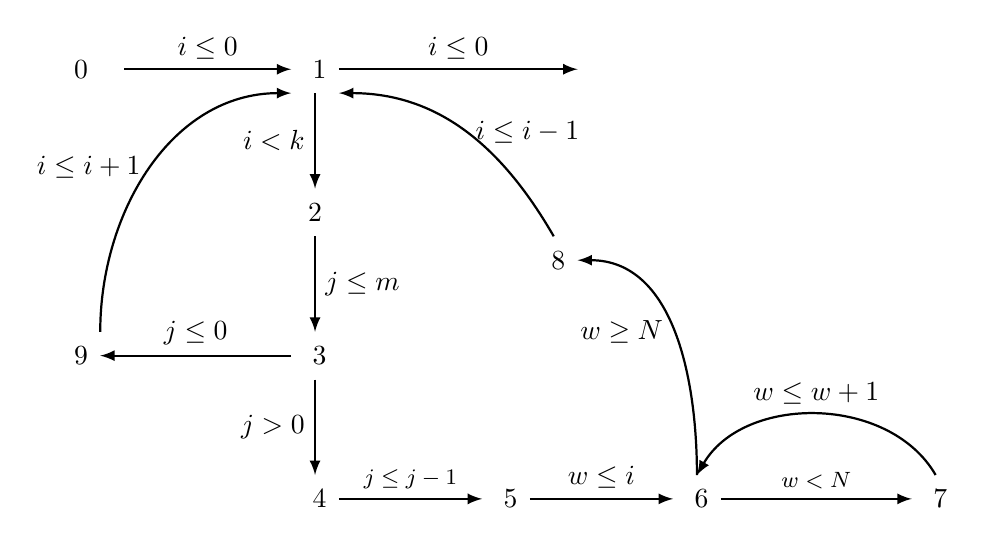
\begin{tikzpicture}[scale=\textwidth/20cm,samples=200]
                \draw[] (-5, 10) circle (0pt) node{{ $0$}};
                \draw[] (0, 10) circle (0pt) node{{ $1$}};
                \draw[] (6, 10) circle (0pt) node {{$\lex$}};
                \draw[] (0, 7) circle (0pt) node{{$2$}};
                \draw[] (0, 4) circle (0pt) node{{ $3$}};
                \draw[] (-5, 4) circle (0pt) node{{ $9$}};
                \draw[] (0, 1) circle (0pt) node{{ $4$}};
                \draw[] (4, 1) circle (0pt) node{{ $5$}};
                \draw[] (8, 1) circle (0pt) node{{ $6$}};
                \draw[] (13, 1) circle (0pt) node{{ $7$}};
                \draw[] (5, 6) circle (0pt) node{{ $8$}};
                % Counter Variables
                %
                % Control Flow Edges:
                \draw[ thick, -latex] (-4, 10)  -- node [above] {$i \leq 0$}(-0.5, 10);
                \draw[ thick, -latex] (0, 9.5)  -- node [left] {$i < k$} (0, 7.5) ;
                \draw[ thick, -latex] (0, 6.5)  -- node [right] {$j \leq m$} (0, 4.5) ;
                \draw[ thick, -latex] (0, 3.5)  -- node [left] {$j > 0$} (0, 1.5) ;
                \draw[ thick, -latex] (-0.5, 4)  -- node [above] {$j \leq 0$} (-4.5, 4) ;
                \draw[ thick, -latex] (-4.5, 4.5)  to  [out=90,in=180]  node [left] {$i \leq i + 1$ }(-0.5, 9.5);
                \draw[ thick, -latex] (0.5, 10)  -- node [above] {$i \leq 0$}  (5.5, 10);
                \draw[ thick, -latex] (0.5, 1)  -- node [above] {{\footnotesize $j \leq j - 1$}}  (3.5, 1);
                \draw[ thick, -latex] (4.5, 1)  -- node [above] {$w \leq i$}  (7.5, 1);
                \draw[ thick, -latex] (8.5, 1)  -- node [above] {{\footnotesize $w < N$}}  (12.5, 1);
                \draw[ thick, -latex] (8, 1.5)  to [out=90,in=0] node [left] {{$w \geq N$}}  (5.5, 6);
                \draw[ thick, -latex] (13, 1.5)  to  [out=120,in=60] node [above] {$w \leq w + 1$}  (8, 1.5);
                \draw[ thick, -latex] (5, 6.5)  to  [out=120,in=0]  node [right] {$i \leq i - 1$ }(0.5, 9.5);
                \end{tikzpicture}
%     \caption{}
%     \end{centering}
%     \end{subfigure}
% \begin{subfigure}{.2\textwidth}    
% \begin{centering}
    {\small
$
    \begin{array}{ll}
        \tpath_0 = (0 \to 1)
        &
        \tpath_4 = (6 \to 8 \to 3)
        \\        
        \tpath_1 = (1 \to 2 \to 3)
        &
        \tpath_5 = (3 \to 9 \to 1)
        \\
        \tpath_2 = (3 \to 4 \to 5 \to 6)
        &
        \tpath_6 = (1 \to \lex)
        \\
        \tpath_3 = (6 \to 7 \to 6)
    \end{array}
$
$
    \begin{array}{l}
        \rprog_1 = {\rprepeat(\tpath_1; 3: {\rprepeat(\tpath_2; 6 : {\rprepeat(\tpath_3)}; \tpath_4)}; \tpath_5)}
        \\
        \rprog_3 = {\rprepeat(\tpath_2; 6 : {\rprepeat(\tpath_3)}; \tpath_4)}
    \end{array}
$
}
\caption{}
\end{centering}
\end{subfigure}
    \caption{
    (a) An example of three nested loops with related iterator variables.
    (b) The abstract transition graph, simple transition paths and loop body.}
        \label{fig:threeWhile-overview}
    \end{figure}

\section{{Program Model}}
\label{sec:language}
\subsection{Language}
\subsection{Trace-Based Operational Semantics}
% \subsection{Labeled Language}
\[
\begin{array}{llll}
\mbox{Arithmetic Operators} 
& \oplus_a & ::= & + ~|~ - ~|~ \times 
%
~|~ \div ~|~ \emax ~|~ \emin
\\  
\mbox{Arithmetic Expression} 
& \aexpr & ::= & 
n ~|~ {x} ~|~ \aexpr \oplus_a \aexpr  
 ~|~ \elog \aexpr  ~|~ \esign \aexpr
\\
\mbox{Boolean Expression} & \bexpr & ::= & 
%
\etrue ~|~ \efalse  ~|~ \neg \bexpr
 ~|~ \bexpr \land \bexpr
%
~|~ \bexpr \lor \bexpr
~|~ \aexpr \leq \aexpr 
~|~ \aexpr < \aexpr 
~|~ \aexpr = \aexpr 
\\
\mbox{Expression} & \expr & ::= & v ~|~ \aexpr ~|~ \bexpr ~|~ [\expr, \dots, \expr]
\\  
%
\mbox{Value} 
& v & ::= & { n \in \mathbb{N}^{\infty} ~|~ \etrue ~|~ \efalse ~|~ [] ~|~ [v, \dots, v]} \\
%
% \\%
\mbox{Label} 
& l & \in & (\mathbb{N} \cup \{\lin, \lex\}) 
\\ 
%
\mbox{Labeled Command} 
& {c} & ::= &  
\clabel{\assign{x}{\expr}}^l 
~|~  \clabel{\eskip}^l
~|~ \ewhile \clabel{\bexpr}^{l} \edo ({c})
~|~ \eif(\clabel{\bexpr}^{l} , {c}, {c}) 
~|~ {c};{c}  
\\ 
\mbox{Event} 
& \event & ::= & 
({x}, l, v) ~ \mbox{Assignment Event} 
% \\
% &&& 
~|~(\bexpr, l, v) ~ \mbox{Testing Event}
\\
\mbox{Trace} & \trace
& ::= & [] ~|~ \trace :: \event
\\
\end{array}
\]
We denote by $\infty$ a value s.t. $n < \infty $ for all $n \in \mathbb{N}$.
We use following notations to represent the sets of corresponding terms:
\[
\begin{array}{lll}
\vardom & : & \mbox{Set of Variables}  
\\ 
%
\booldom & : & \mbox{Set of Boolean Expressions}  
\\ 
%
\cdom & : & \mbox{Set of Commands} 
\\ 
%
\eventset  & : & \mbox{Set of Events}  
\\
%
\eventset^{\asn}  & : & \mbox{Set of Assignment Events}  
\\
%
\eventset^{\test}  & : & \mbox{Set of Testing Events}  
\\
%
\ldom  & : & \mbox{Set of Labels}  
\\
%
\highlight{\ftdom} & : & \mbox{\highlight{Set of All Finite Execution Traces}}
\\
\highlight{\inftdom} & : & \mbox{\highlight{Set of Infinite  Execution Traces}}
\\
\highlight{\tdom} & : & \mbox{\highlight{Set of All Finite Or Infinite  Execution Traces}}
\\ 
%
\inpvar(c) & : & \mbox{Set of Program $c$'s Input Variables}  
\\
%
\ftdom_0(c) & : & \mbox{Set of Program $c$'s Initial Traces.}
\\ & & \mbox{Each initial trace $\trace_0 \in \ftdom_0(c)$ is finite and every input variable of the program $c$ has an initial value in $\trace_0$.}
\end{array}
\]
%
\subsection{{Trace-based Operational Semantics}}
\label{sec:operational_semantics}
\paragraph{Event}
An event is a triple.
Its first element is the variable name $x$,
or a boolean expression (from the guard of if or while command), 
following by 
 the label, $l$ associated to this command and the value assigned to the variable.

 We have two kinds of events: \emph{assignment events} and \emph{testing events},
 and we use $\eventset^{\asn}$ and $\eventset^{\test}$ to denote the set of all assignment events and testing events, respectively.

 An \emph{assignment event} tracks the execution of an assignment and consists of the assigned variable, the label of the command that generates it, the value assigned to the variable.

 A \emph{testing event} tracks the execution of if and while commands, specifically the evaluation of the boolean expression $b$ in the guard of a $\eif(\clabel{b}^l, c_1, c_2)$ command or $\ewhile \clabel{b}^l \edo c$.
 It consists of the boolean expression $b$ in the guard of the command, the label of the guard, the result of evaluating the guard.
%
\[
\begin{array}{llll}
  \mbox{Event} 
  & \event & ::= & 
  ({x}, l, v) ~ \mbox{Assignment Event} 
  ~|~(\bexpr, l, v) ~ \mbox{Testing Event}
\end{array}
\]
Event projection operators $\pi_i$ projects the $i^{th}$ element from an event: 
% \\
$\pi_i : 
\eventset \to \vardom \cup \booldom \cup \ldom $

\paragraph{Trace.}
%
A trace $\trace \in \tdom $ is a list of events, 
collecting the events generated along the program execution. 
\[
\begin{array}{llll}
\mbox{Trace} & \trace
& ::= & [] ~|~ \trace :: \event
\end{array}
\]
A trace can be regarded as the program history, 
which records all the evaluations for assignment commands and guards in $\eif$ and $\ewhile$ command.
\\
\highlight{If a program doesn't terminate when executing under some initial trace, it produces an infinite trace $\trace \in \tdom^{\infty}$.
$\tdom^{\infty}$ is the set of all finite or infinite traces.}
\\
$\tracecat: \mathcal{T} \to \mathcal{T} \to \mathcal{T}$ is the trace concatenation operator, which combines two traces,
and $\vcounter : \mathcal{T} \to \mathbb{N} \to \mathbb{N}$ is the counting operator, 
which counts the occurrence of a labeled variable in the trace. When the input trace is infinite, it returns $\infty$.
$\event \in \trace $ or $\event \notin \trace $ denotes that $\event$ belongs to $trace$ or not.
All the definition details are in the appendix.
%
The counter operator is abused when the input is a sequence of labels $L = (l_1, \cdots, l_n)$ by counting the occurrence
of this sequence in trace. Specifically,
$\vcounter(\trace :: (\_, l_1, \_) :: \cdots :: (\_, l_n, \_), L ) \triangleq \vcounter(\trace, L) + 1$
and $\vcounter(\trace :: (\_, l, \_), L ) 
\triangleq \vcounter(\trace, L) ~ l \neq l_n$, etc.
The operator $\tlabel : \tdom \to \mathcal{P}{(\ldom)}$ gives the set of labels in every event belonging to a trace.
$\tlabel{(\trace  :: (\_, l, \_)])} \triangleq \{l\} \cup \tlabel{(\trace )}$ and $\tlabel({[ ]}) \triangleq \{\}$.
%
\paragraph{Environment.} $\env : {\ftdom}  \to \vardom \to(\mathbb{N} \cup \{\bot\})$
\[
\begin{array}{llll}
\env(\trace  \traceadd (x, l, v)) x \triangleq v
&
\env(\trace \traceadd (y, l, v)) x \triangleq \env(\trace) x, y \neq x
&
\env(\trace \traceadd (b, l, v)) x \triangleq \env(\trace) x
&
\env({[]} ) x \triangleq \bot
\end{array}
\]
%
\begin{lem}[Initial Traces]
  \label{lem:initial_trace}
  \[
    \forall c \in \cdom, \trace \in \ftdom \st \trace \in \ftdom_0(c) \iff 
    \forall x \in \inpvar(c) \st \env(\trace_0) x \neq \bot
    \]
\end{lem}
%
\paragraph{Configuration.}
%
\paragraph{Expression Semantics}
The evaluation notation for arithmetic expression is $\econfig{} : \mathcal{A} \to \tdom \to \mathcal{V}$.
The $\econfig{\aexpr}(\trace)$ evaluates an arithmetic expression $\aexpr$ under trace $\trace$ following the arithmetic expression evaluation rules in Figure~\ref{fig:aexpr-eval}.
\begin{figure}
\begin{mathpar}
  \boxed{ \econfig{} \, : \, \mbox{Arithmetic Expression $\to$ Trace $\to$ Arithmetic Value}}
  \\
  \inferrule{ 
    \empty
  }{
   \econfig{n} (\trace)
   = n
  }
  \and
  \inferrule{ 
    \env(\trace) x = v
  }{
   \econfig{x} 
   = v
  }
  \and
  \inferrule{ 
    \econfig{\aexpr_1}(\trace) = v_1
    \and 
    \econfig{\aexpr_2}(\trace) = v_2
    \and 
     v_1 \oplus_a v_2 = v
  }{
   \econfig{\aexpr_1 \oplus_a \aexpr_2} 
   = v
  }
  \and
  \inferrule{ 
    \econfig{\aexpr}(\trace) = v'
    \and 
    \elog v' = v
  }{
   \econfig{\elog \aexpr}(\trace) 
   = v
  }
  \and
  \inferrule{ 
    \econfig{\aexpr}(\trace) = v'
    \and 
    \esign v' = v
  }{
   \econfig{\esign \aexpr} 
   = v
  }
   \end{mathpar}
   \caption{Evaluation Rules of Arithmetic Expression}
   \label{fig:aexpr-eval}
   \end{figure}

 The evaluation rules for boolean expression and standard expression are in Figure~\ref{fig:bexpr-eval} and Figure~\ref{fig:expr-eval}.
 \begin{figure}
  \begin{mathpar}
  \boxed{ \barrow \, : \, \mbox{ Boolean Expression $\times$ Trace $\rightarrow$ Boolean Value} }
  \\
  \inferrule{ 
    \empty
  }{
   \config{\efalse, \trace} 
   \barrow \efalse
  }
  \and 
  \inferrule{ 
    \empty
  }{
   \config{\etrue, \trace} 
   \barrow \etrue
  }
  \and 
  \inferrule{ 
    \config{\bexpr, \trace} \barrow v'
    \and 
    \neg v' = v
  }{
   \config{\neg \bexpr, \trace} 
   \barrow v
  }
  \and 
  \inferrule{ 
    \config{\bexpr, \trace_1} \barrow v_1
    \and 
    \config{\bexpr, \trace_2} \barrow v_2
    \and 
     v_1 \land v_2 = v
  }{
   \config{\bexpr, \trace_1 \land \bexpr_2} 
   \barrow v
  }
  \and 
  \inferrule{ 
    \config{\bexpr, \trace_1} \barrow v_1
    \and 
    \config{\bexpr, \trace_2} \barrow v_2
    \and 
     v_1 \lor v_2 = v
  }{
   \config{\bexpr, \trace_1 \lor \bexpr_2} 
   \barrow v
  }
  \end{mathpar}
  \caption{Evaluation Rules of Boolean Expression}
  \label{fig:bexpr-eval}
  \end{figure}
  
  \begin{figure}
    \begin{mathpar}
  \boxed{ \earrow \, : \, \mbox{Expression $\times$ Trace $\rightarrow$ Value} }
  \\
  \inferrule{ 
    \econfig{\aexpr}(\trace) = v
  }{
   \config{\aexpr, \trace} 
   \earrow v
  }
  \and
  \inferrule{ 
    \config{\bexpr, \trace} \barrow v
  }{
   \config{\bexpr, \trace} 
   \earrow v
  }
  \and
  \inferrule{ 
    \config{\expr_1, \trace} \earrow v_1
    \cdots
    \config{\expr_n, \trace} \earrow v_n
  }{
   \config{ [\expr_1, \cdots, \expr_n], \trace} 
   \earrow [v_1, \cdots, v_n]
  }
  \and
  \inferrule{ 
    \empty
  }{
   \config{v, \trace} 
   \earrow v
  }
   \end{mathpar}
   \caption{Evaluation Rules of Standard Expression}
   \label{fig:expr-eval}
   \end{figure}

\paragraph{Operational Semantics Rules}
%
The trace based operational semantics rules are defined as in Figure~\ref{fig:command-os}.
\begin{figure}
  \begin{mathpar}
\boxed{
\mbox{Command $\times$ Trace}
\xrightarrow{}
\mbox{Command $\times$ Trace}
}
\and
\boxed{\config{{c, \trace}}
\xrightarrow{} 
\config{{c',  \trace'}}
}
%
\\
%
\inferrule
{
\config{\expr, \trace} \earrow v
  \and
\event = ({x}, l, v)
}
{
\config{\clabel{\assign{{x}}{\expr}}^{l},  \trace } 
\xrightarrow{} 
\config{\clabel{\eskip}^l, \trace \traceadd \event}
}
~\rname{assn}
\and
%
\inferrule
{
  \config{\bexpr, \trace} \earrow \etrue
 \and 
 \event = (\bexpr, l, \etrue)
}
{
\config{{\ewhile \clabel{\bexpr}^{l} \edo (c), \trace}}
\xrightarrow{} 
\config{{
c; \ewhile \clabel{\bexpr}^{l} \edo (c),
\trace \traceadd \event}}
}
~\rname{while-t}
%
%
\and
%
\inferrule
{
  \config{\bexpr, \trace} \earrow \efalse
 \and 
 \event = (\bexpr, l, \efalse)
}
{
\config{{\ewhile \clabel{\bexpr}^{l} \edo (c), \trace}}
\xrightarrow{} 
\config{{
  \clabel{\eskip}^l,
\trace \traceadd \event}}
}
~\rname{while-f}
%
%
\and
%
%
\inferrule
{
\config{{c_1, \trace}}
\xrightarrow{}
\config{{c_1',  \trace'}}
}
{
\config{{c_1; c_2, \trace}} 
\xrightarrow{} 
\config{{c_1'; c_2, \trace'}}
}
~\rname{seq1}
%
\and
%
\inferrule
{
  \config{{c_2, \trace}}
  \xrightarrow{}
  \config{{c_2',  \trace'}}
}
{
\config{{\clabel{\eskip}^l; c_2, \trace}} \xrightarrow{} \config{{ c_2', \trace'}}
}
~\rname{seq2}
%
\and
%
%
\inferrule
{
  \config{\bexpr, \trace} \earrow \etrue
 \and 
 \event = (\bexpr, l, \etrue)
}
{
\config{{
\eif(\clabel{\bexpr}^{l}, c_1, c_2), 
\trace}}
\xrightarrow{} 
\config{{c_1, \trace \traceadd \event}}
}
~\rname{if-t}
%
\and
%
\inferrule
{
 \config{\bexpr, \trace} \earrow \efalse
 \and 
 \event = (\bexpr, l, \efalse)
}
{
\config{{\eif(\clabel{\bexpr}^{l}, c_1, c_2), \trace}}
\xrightarrow{} 
\config{{c_2, \trace \traceadd \event}}
}
~\rname{if-f}
%
\end{mathpar}
\caption{Operational Semantics Rules}
\label{fig:command-os}
\end{figure}


Given an initial trace $\trace_0 \in \ftdom_0(c)$ of the program $c$,
we use $\to^*$ for the reflexive and transitive closure of $\to$. 
If $\config{c, \trace_0} \rightarrow^{*} \config{\clabel{\eskip}^l, \trace_0 \tracecat \trace}$,
then the program's execution terminates and produces a finite execution trace $\trace \in \ftdom$.
\\
\begin{defn}[Non-terminating and Infinite Trace]
  \label{def:non-terminating}
  Given a program $c$ and an initial trace $\trace \in \ftdom_0(c)$,
  when $c$ executes with $\trace$,  we define the execution of $c$ under $\trace$ is non-terminating and produces an infinite trace $\trace' \in \inftdom$, as 
  $\config{c, \trace_0} \uparrow^{\infty} \trace' \in \lim(\uparrow)$
  where the limit is defined as follows.
  \[
    \begin{array}{l}
      \lim(\uparrow) 
      % \in \left( (\cdom \times \ftdom) \times (\cdom \times \inftdom) \right) 
      \triangleq 
    \\ \quad
    \Big\{
      (\config{c, \trace}, \trace') ~\vert~ 
      c\in \cdom, \trace \in \ftdom_0(c),
      \trace' \in \inftdom 
      \land \exists \trace_0 \in \ftdom, c_0 \in \cdom \st 
      \config{c, \trace} \to \config{c_0, \trace_0}
      \\ \qquad \qquad \qquad 
      \land \forall i \in \mathbb{N}, \exists \trace_i, \trace_{i + 1} \in \ftdom, \trace'' \in \inftdom, c_i, c_{i + 1} \in \cdom \st 
      \config{c_i, \trace_i} \to \config{c_{i + 1}, \trace_{i + 1}} 
      \land  \trace' = \trace_{i + 1} \tracecat \trace''
    \Big\}
    \end{array}
  \]
\end{defn}
%
% \begin{defn}[Non-terminating and Infinite Trace (alternative way)]
%   \label{def:non-terminating-2}
%   Given a program $c$ and an initial trace $\trace_0 \in \ftdom_0(c)$,
%   when $c$ executes with $\trace_0$,  we define $c$ is non-terminating under $\trace_0$, $\config{c, \trace_0} \uparrow^{\infty}$ if and only if there exists a function
%   $f : \mathbb{N} \to \cdom \times \tdom$ such that $f(0) = \config{c, \trace_0}$ and
%   for every $i \in \mathbb{N}$ there exist  $\trace_i, \trace_{i + 1}\in \tdom$, $c_i, c_{i + 1} \in \cdom$ such that  $f(i) = \config{c_i, \trace_i}$, $f(i + 1) =  \config{c_{i + 1}, \trace_{i + 1}}$ and
%   $\config{c_i, \trace_i} \to \config{c_{i + 1}, \trace_{i + 1}}$. 
%   \[
%     \begin{array}{l}
%     \forall \trace_0 \in \ftdom_0(c), c \in \cdom \st
%     \config{c, \trace_0} \uparrow^{\infty}
%     \\
%     \iff \exists f : \mathbb{N} \to \cdom \times \tdom \st 
%     f(0) = \config{c, \trace_0}
%     \\ \qquad \land
%     \forall i \in \mathbb{N}, \exists \trace_i, \trace_{i + 1} \in \tdom, c_i, c_{i + 1} \in \cdom\st 
%     \\ \qquad \quad
%     f(i) = \config{c_i, \trace_i}$, $f(i + 1) =  \config{c_{i + 1}, \trace_{i + 1}} \land \config{c_i, \trace_i} \to \config{c_{i + 1}, \trace_{i + 1}}
%     \end{array}
%   \]
%   Given a program $c$ and an initial trace $\trace_0 \in \ftdom_0(c)$, if $\config{c, \trace_0} \uparrow^{\infty}$, 
%   let $f$ be the function such that for every $i \in \mathbb{N}$,  $\trace_i, \trace_{i + 1}\in \tdom$, $c_i, c_{i + 1} \in \cdom$ where $\config{c_i, \trace_i} \to \config{c_{i + 1}, \trace_{i + 1}}$, we have $f(i) = \config{c_i, \trace_i}$, $f(i + 1) =  \config{c_{i + 1}, \trace_{i + 1}}$. 
%   Let $\pi_2 : (\cdom \times \tdom) \to \tdom$ be the projector which projects the trace from a configuration,
%   then we define $\config{c, \trace_0} \uparrow^{\infty} \trace'$ produces an infinite trace $\trace' = \pi_2(\lim\limits_{i \to \infty}(f(i))) \in \inftdom$.
%   \[ \trace' = \lim( \pi_2 \circ (f(i))). \]
% \end{defn}
% %

% \begin{defn}[Non-terminating and Infinite Trace (third way)]
%   \label{def:infinite-trace}
%   Given a program $c$ and an initial trace $\trace_0 \in \ftdom_0(c)$,
%   when $c$ executes with $\trace_0$,  we define $c$ is non-terminating under $\trace_0$, denoted as $\config{c, \trace_0} \uparrow^{\infty} \trace'$ and produce an infinite trace $\trace' \in \inftdom$ 
%   if and only if there exists a function
%   $f : \mathbb{N} \to \cdom \times \tdom$ such that $f(0) = \config{c, \trace_0}$ and
%   for every $i \in \mathbb{N}$ there exist  $\trace_i, \trace_{i + 1}\in \tdom$, $c_i, c_{i + 1} \in \cdom$ such that  $f(i) = \config{c_i, \trace_i}$, $f(i + 1) =  \config{c_{i + 1}, \trace_{i + 1}}$ and
%   $\config{c_i, \trace_i} \to \config{c_{i + 1}, \trace_{i + 1}}$. 
%   \[
%     \begin{array}{l}
%     \forall \trace_0 \in \ftdom_0(c), \trace' \in \inftdom, c \in \cdom \st
%     \config{c, \trace_0} \uparrow^{\infty} \trace'
%     \\
%     \iff \exists f : \mathbb{N} \to \cdom \times \tdom \st 
%     f(0) = \config{c, \trace_0}
%     \\ \qquad \land
%     \forall i \in \mathbb{N}, \exists \trace_i, \trace_{i + 1} \in \tdom, c_i, c_{i + 1} \in \cdom\st 
%     \\ \qquad \quad
%     f(i) = \config{c_i, \trace_i}$, $f(i + 1) =  \config{c_{i + 1}, \trace_{i + 1}} \land \config{c_i, \trace_i} \to \config{c_{i + 1}, \trace_{i + 1}}.
%     \end{array}
%   \]
%   Let $\pi_2 : (\cdom \times \tdom) \to \tdom$ be the projector which projects the trace from a configuration,
%   then the infinite trace $\trace'$ produced by $\config{c, \trace_0} \uparrow^{\infty} \trace'$ is
%   \[ \trace' = \pi_2(\lim\limits_{i \to \infty}(f(i))) \in \inftdom. \]
% \end{defn}
%
This follows the maximal trace semantics in \cite{cousot2019abstract} Section 2.5 Equation (12).
\\
If we observe the operational semantics rules, we can find that no rule will shrink the trace. 
So we have the Lemma~\ref{lem:tracenondec} with proof in Appendix~\ref{apdx:lem_language}, 
specifically the trace has the property that its length never decreases during the program execution.
\begin{lem}
  [Trace Non-Decreasing]
  \label{lem:tracenondec}
  For any program $c \in \cdom$ and initial trace $\trace_0 \in \ftdom_0(c)$,
  if there exists $\trace \in \tdom$ and $c' \in \cdom $ such that $\config{c, \trace_0} \rightarrow^{*} \config{c', \trace} $ or 
  $\config{c, \trace_0} \uparrow^{\infty} \trace$  
  then there exists a trace $\trace' \in \tdom$ such that $\trace_0 \tracecat \trace' = \trace$ formally as follows.
  %
  \[
    \begin{array}{l}
    \forall \trace_0 \in \ftdom_0(c), \trace \in \tdom, c, c' \in \cdom \st
    \Big( \config{c, \trace_0} \rightarrow^{*} \config{c', \trace} 
    \lor  \config{c, \trace_0} \uparrow^{\infty} \trace \Big)
    \\ \quad
    \implies \exists \trace' \in \tdom \st \trace_0 \tracecat \trace' = \trace 
    \end{array}
    \]
  \end{lem}
  % \begin{lem}
  %   [Trace Non-Decreasing (based on the alternative non-termination definition)]
  %   \label{lem:tracenondec2}
  %   For any program $c \in \cdom$ and initial trace $\trace_0 \in \ftdom_0(c)$,
  %   \begin{itemize}
  %     \item if there exists $\trace \in \tdom$ and $c' \in \cdom $ such that $\config{c, \trace_0} \rightarrow^{*} \config{c', \trace} $
  %     then there exists a trace $\trace' \in \ftdom$ such that $\trace_0 \tracecat \trace' = \trace$;
  %     \item if $\config{c, \trace_0} \uparrow^{\infty} $ and produces an infinite trace $\trace \in \inftdom$ as defined in Definition~\ref{def:non-terminating}
  %     then there exists an infinite trace $\trace' \in \inftdom$ such that $\trace_0 \tracecat \trace' = \trace$ formally as follows.  
  %   \end{itemize}
  %   %
  %   \[
  %     \begin{array}{l}
  %     \forall \trace_0 \in \ftdom_0(c), \trace \in \tdom, c, c' \in \cdom \st
  %     \config{c, \trace_0} \rightarrow^{*} \config{c', \trace} 
  %     \implies \exists \trace' \in \ftdom \st \trace_0 \tracecat \trace' = \trace 
  %     \\
  %     \todomath{\land \config{c, \trace_0} \uparrow^{\infty} \implies \exists \trace' \in \inftdom \st \trace_0 \tracecat \trace' \in \inftdom}
  %     \end{array}
  %     \]
  %   \end{lem}
% %
% %
\subsection{{Reachability Bound}}
\label{sec:execution_rb}
% %
\begin{defn}[Execution Based Reachability Bound]
\label{def:trace_graph}
Given a program ${c}$,
its \emph{Execution-Base Reachability Bound} 
$\exeRB({c})$ is defined as follows,
% over all possible traces,
%
\highlight{
\[
\begin{array}{lcl}
  % \text{Vertices} &
  \exeRB({c}) & := & 
  \{ 
  (l, w) 
  ~ \vert ~ 
  w : \mathcal{T} \to \mathbb{N}
  \land
  l \in \lvar(c) 
  \\ & &
  \land
  \forall \trace \in \mathcal{T}_0(c), \trace' \in \mathcal{T} \st \config{{c}, \trace} \to^{*} \config{\eskip, \trace\tracecat\vtrace'} 
  \implies w(\trace) = \vcounter(\vtrace', l) 
\}
\end{array}
\]
}
\end{defn}
There are two components.
\\
In most data analysis programs c we are interested, there are usually some user input variables,
such as $k$ in Example~\ref{ex:whileOdd}. We denote $\mathcal{T}_0(c)$ as the set of initial traces in which all the input variables in
$c$ are initialized
\highlight{
The $\exeRB(c)$  is a set of pairs, $(x^l, w) \in \mathcal{LV} \times (\mathcal{T} \to \mathbb{N})$,
with a labeled variable as first component and
its weight $w$ the second component.
Weight $w$ for
% a labeled variable 
$x^l$ is a function $w : \mathcal{T} \to \mathbb{N}$
mapping from a starting trace to a natural number.
When program executes under this starting trace $\trace$,
$\config{{c}, \trace} \to^{*} \config{\eskip, \trace\tracecat\vtrace'} $, it generates an execution trace $\trace'$.
This natural number is the evaluation times of the labeled command corresponding to the vertex, 
computed by the counter operator $w(\trace) = \vcounter(\vtrace', l)$.
We can see in the execution-based dependency graph of $\kw{twoRounds}$ in
 Figure~3(b) in main paper, the weight of vertices in the while loop is  $\env(\trace) k$, 
 which depends on the value of the user input $k$ specified in the starting trace $\tau$.
}
% it is also reflected in $\traceW({c})$.   
% % 
\section{Path Sensitive Reachability Bound Analysis}
\label{sec:psrb-alg}
% % In this section, we present our algorithm for computing the upper bound for a program $c$'s adaptivity
% $A(c)$ defined~\ref{def:trace_adapt} through static program analysis.
% This section presents the key definitions
% for the static analysis algorithm in Section~\ref{sec:algorithm-keys} before going into the detail of the algorithm,
% then shows the complete static analysis algorithm.
% \mg{
% In this section, we present our static program analysis for computing an upper bound on the adaptivity a program $c$
% }
In this section, we present our static program analysis for computing an upper bound on the 
execution-based reachability times for every label $l$ of an arbitrary program $c$.
% , as defined in last section.
%
\subsection{Algorithm Overview}
\label{sec:alg_overview}
In order to have the upper bound of the reachability for every label of a program $c$, we design 
a path sensitive reachability bound analysis algorithm {\THESYSTEM}.
It can be summarized as the following steps: 
% \begin{figure}
%   \centering    
% \includegraphics[width=1.0\columnwidth]{adapfun.png}
%   \vspace{-0.3cm}
%   \caption{The overview of {\THESYSTEM}}
%   \label{fig:adaptfun}
%   \vspace{-0.5cm}
% \end{figure}
%
%
\begin{enumerate}
\item  In Section~\ref{sec:abscfg}, we first construct an abstract control flow graph based on $c$, by computing an abstract transition 
for every labeled command. 
This graph is used in Section~\ref{sec:reachabilitybound_algorithm} for analyzing program's reachability bound.
% see Section~\ref{sec:alg_vertexgen}
\item The Section~\ref{sec:reachabilitybound_algorithm} computes program's reachability bound in two steps as follows.
\begin{enumerate}
\item The Section~\ref{sec:pathinsensitive_rb} estimates path-insensitive reachability upper bound for every while loop command in $c$.
% Vertices are the assigned variables with unique labels, which is extracted directly from the program, 
% Every vertex come with a weight, which tells the maximal times each vertex and edge can be visited in realistic execution. This weight is estimated by a reachability bound analysis on each vertex, See Section~\ref{sec:alg_weightgen}.
% \item Each edge also vertices considers both control flow and data flow, See
% Section~\ref{sec:alg_edgegen}
\item The Section~\ref{sec:pathsensitive_rb} estimates the path-sensitive reachability upper bound 
for every program locations (i.e., every command label) through four steps:
\begin{enumerate}
\item {\THESYSTEM} firstly refines this program into the rephrased and refined program, based on the abstract control flow graph
generated in Section~\ref{sec:abscfg}.
\item Then in the second and third steps, it performs the Outside-In and Inside-Out Algorithms 
on this refined program, and obtains 
path-sensitive reachability bound for each edge on the abstract control flow graph.
\item At the last step, {\THESYSTEM} computes the path-sensitive reachability bound for every label in this program $c$ by summarizing 
the path-sensitive reachability bound of each edge on the abstract control flow graph.
\end{enumerate}
\end{enumerate}
% Finally, with all the ingredients ready, we construct the final approximated program-based dependency graph in Section~\ref{sec:alg_graphgen}
\end{enumerate}

% the algorithm  without extra static analysis technique.
% \\
% Overall, this program-based graph has a similar topology structure as 
% % the one
% % of 
% the Execution-Based Dependency Graph. It has the same
% vertices and query annotations, but approximated edges and weights. We call the graph generated by static analysis techniques, static analysis dedendency graph. 
% \item Then in the last phase in Section~\ref{sec:alg_adaptcompute}, $\THESYSTEM$
% % we compute the upper bound for adaptivity over this approximated graph:
% % , as an upper bound for
% % program's adaptivity
% computes the upper bound for adaptivity over this approximated graph.
% in the last phase of this algorithm in Section~\ref{sec:alg_adaptcompute}.
% \subsection{Adaptivity Based on Program Analysis in \THESYSTEM}
% In order to give a bound on the program's adaptivity, we first build a
% program-based data-dependency graph to {over-}approximate the
% trace-based dependency graph.  Then, we define a program-based
% adaptivity over this approximated graph, as an upper bound for
% $A(c)$.
% %
% \subsection{ $\THESYSTEM$ Analysis Algorithm}
% \subsection{Dependency Graph Estimation}
% \subsection{Vertices Estimationn}
% \label{sec:alg_vertexgen}
% The first component of every vertex in the static analysis dependency graph are actually identical as the  Execution-Based Dependency Graph, which are assigned variables in the program annotated with the unique label(line number). 
% These vertices are collected by statically scanning the program, like what we do for vertices of its Execution-Based Dependency Graph. 
% The vertices are defined formally as follows.

%   \highlight{
% \[
%     \progV^0(c) \triangleq \left\{ 
%   (x^l, w) \in \mathcal{LV} \times \mathcal{A}_{\lin}
%   ~ \middle\vert ~
%   x^l \in \lvar(c)
%   \right\}
%   \]
%   }
%   %
% where $\mathcal{A}_{\lin}$ is the set of arithmetic expressions over $\mathbb{N}$ and program's input variables. 
% The weight $w$ for every vertex will be computed in following step in Section~\ref{sec:alg_weightgen}.
% The static scanning of the programs also tells us whether one vertice(assigned variable) is assigned by a query request. We have similar definition when defining the Execution-Based Dependency Graph, 
% a set of pairs $\progF(c) \in \mathcal{P}(\mathcal{LV} \times \{0, 1\} )$ 
% % is the set of pairs 
% % The weight for each vertex in $\progV(c)$ is computed 
% mapping each $x^l \in \progV(c)$ to a flag, either $0$ or $1$, where $1$  means $x^{l}$ is a member of $ \qvar_{c}$, a set of those variables assigned with query requests, and $0$ means $x^{l}$ not in this set. It is defined formally below.

% \[\progF(c) =\left\{(x^l, n)  \in  \mathcal{LV} \times \{0, 1\} 
% ~ \middle\vert ~
% x^l \in \lvar_{c},
% n = 1 \iff x^l \in \qvar_{c} \land n = 0 \iff  x^l \not\in \qvar_{c} .
% \right\}\]
%

% \wq{To do: Add $\THESYSTEM$, a data flow analysis algorithm to scan the program and give a graph.}
% {\THESYSTEM} consists of three phases: 
% \begin{enumerate}
%     \item Generating an abstract control flow graph with each edge representing an abstract event transiting between two command labels. 
%     \item Computing the value bound invariant for each variable in the event and 
%     the event transition closure over the abstract control flow graph,
%     we get the reachability bound for each labeled command.
%     \item Refining the abstract control flow graph with data-flow, by performing the reaching definition analysis, we generate a weighted data control flow graph.
%     \item An algorithm to find the appropriate path in the weighted data control flow graph
% \end{enumerate}

% \begin{enumerate}
%     \item An algorithm to generate a precise data control flow graph
%     \item An algorithm to perform a Reachability number analysis to calculate the weight of each node in the graph generated in phase 1.
%     \item An algorithm to find the appropriate path in the weighted data control flow graph
% \end{enumerate}

% \subsection{Edge and Weight Estimation}
% \label{sec:alg_weightedgegen}

% Since the edges of the execution-based graph of a program relies on the dependency relation, which handles both control flow and data flow, as an over-approximation of this graph, the edges of our static anlaysis dependency graph also covers these two kind of flows. We develop a feasible data flow relation to catch these two flows, in Section~\ref{sec:alg_edgegen}.


% The weight of every vertice in the execution-based graph is built on all possible execution traces.
% In order to over-approximate the weight statically but still tightly, we present a symbolic reachability bound analysis for estimation of the weight of each vertice(label) in Section~\ref{sec:alg_weightgen},
% in spirit of some reachablility bound techiniques.


% The edges and weight estimation are both performed on basis of an abstract control flow graph of the program, we first show how to generate this abstract execution control flow graph before the introduction of  the edge and weight estimation.  

% This analysis first 
%  generate an abstract control flow graph
%  over all program labels, 
% in order to analyzing the data flow relations through variables assigned in every labeled command,
% and the reaching time of each variable.
% Then, it refines this control flow graph 
% % into a weighted data-dependency graph, 
% and generate the Program-Based Dependency Graph,
% through the data flow and reaching bound analysis results.
% In the last step, it finds the longest finite walk in this weighted data control flow graph w.r.t. the query variables,
% and return the number of query vertices traversed alongside.
% % \wq{To do: Add $\THESYSTEM$, a data flow analysis algorithm to scan the program and give a graph.}
% To be more specific, {\THESYSTEM} consists of five phases as follows,
% \\
% % \jl{Better to have a graph or picture of overview of the algorithm}
% \todo{graph}
% \todo{pass again}
% This analysis
% \begin{enumerate}
%     % \item Generating 
%     \item first generate 
%     an abstract control flow graph
%     %  over all labels,
%     (remove?? with program's labels as vertices and abstract transitions as edges)
%     in Section~\ref{sec:abscfg},
%     % used to analyze 
%     for analyzing the weight of every vertex in $\progV(c)$ and edges between every vertex in $\progV(c)$ in the next two steps;
%     %  \ref{sec:alg_weightgen} and 
%     % \ref{sec:alg_edgegen}.

%     % which are used as program's control locations,
%     %
%     \item then use the abstract control flow graph generated above, 
%     compute the weight of every vertex in $\progV(c)$ by computing a symbolic reachability bound for each label in Section~\ref{sec:alg_weightgen},
%     % \\
%     \item and then use the same graph again to estimate the edges between every vertex in $\progV(c)$ by computing the feasible data flow relation between every labeled variables in Section~\ref{sec:alg_edgegen}.
  
% \end{enumerate}

\subsection{Abstract Execution Control Flow graph}
\label{sec:abscfg}

This estimation is performed on basis of an abstract control flow graph of the program, 
we first show how to generate this abstract execution control flow graph before the introduction of  the edge and weight estimation.  
We discuss the vertices and edge of the
abstract control flow graph for a program $c$, $\absG(c)$.

\subsubsection{Vertices Construction}
\label{sec:abscfg-vertex}
Every 
vertex corresponds to the unique
label.
Specifically,
the vertices of this graph is the set of $c$'s labels with the exit label ${\lex}$, 
\[ 
  \absV(c) = \lvar(c)\cup\{{\lex}\}
  \]
%  corresponding to a label command in the program.

\subsubsection{Edge Construction}
\label{sec:abscfg-edge}
  The edge in the abstract control flow graph comes from the abstract execution trace of the program. 
  The abstract execution trace, an abstract representation of the execution, consists of a list of abstract transitions. 
  Then, every abstract transition in the abstraction execution trace corresponds to an edge in the abstract control flow graph. In another word, the edge $(l_1, dc, l_2)$ in the abstract control flow graph, represents an abstract transition 
 from $l_1$ to $l_2$, with a set of difference constraints $dc$. 
 Also notice, the difference constraints generated during the abstract transition appears in the edge as annotation.

  Overall, the vertices can be easily collected and the key point of construction of the abstract execution control flow graph for a program is the abstract execution trace, 
  which relies on the abstraction of expression and abstract transition (we also call it abstract event), we will discuss in the following section.
   To make it easy to understand, abstract control flow graph is a control flow graph, with difference constraints on every edge.

%
\paragraph*{Expression Abstraction}

The expression assigned to the variable on the left hand of the assignment command is abstracted to an abstract value: (adopted from the expression abstraction method in paper \cite{sinn2017complexity}). The abstract value is expressed in the form of Difference constraint, denotated as $DC : \mathcal{VAR} \cup \constdom \to \mathcal{\mathcal{VAR} \times (\mathcal{VAR} \cup \constdom) } \times (\mathbb{Z} \cup \{\infty\})$.  $\constdom$ is called the Symbolic Constant defined as $\constdom \triangleq \mathbb{N} \cup \inpvar$
%  \cup \{\max{(\dbdom)}\} $, 
which consists of 
natural numbers $\mathbb{N}$,
the program's input variables $\inpvar$. 
% and a constant value $Q_m$ for estimating the upper bound of variables which are
% assigned by queries. 

Give an instance of difference constraint used here,
$DC(\mathcal{VAR}  \cup \constdom) \cup \{\top\}$ represents all the difference constraints over 
variable and symbolic constants. 
% The difference constraint $DC$ over $\mathcal{VAR} \cup \constdom$ 
It is a set of the inequality of form $x \leq y + v$ where $x \in \mathcal{VAR} $, 
$y \in \mathcal{VAR}  \cup \constdom$ and $v \in \mathbb{Z}$. 
This difference constraint is defined in the same way as
\cite{sinn2017complexity}. For concise, we use $\dcdom^{\top}$ to represent the $DC(\mathcal{VAR}  \cup \constdom) \cup \{\top\} \cup \mathcal{BEXPR}$.

We show the expression abstraction $\absexpr : \expr \to \mathcal{VAR} \to \dcdom^{\top} $ below.

% We introduce the following notations and operations first
% % an expression abstraction method based on the expression abstraction in paper \cite{sinn2017complexity}.
% \\
% % is enriched into $\constdom \triangleq \mathbb{N} \cup \inpvar \cup \{\max{(\dbdom)}\} $.
% T
% \\

% represents the set of inequality over all $\mathcal{VAR}  \cup \constdom$. 

% The symbolic constant is enriched into $\constdom \triangleq \mathbb{N} \cup \inpvar \cup \{\max{(\dbdom)}\} $.
% It consists of 
% natural number $\mathbb{N}$,
% the symbolic constants $\inpvar$ (i.e., the set of the program's input variables), 
% and a constant value $Q_m$ for estimating the upper bound of variables which are
% assigned by queries.
% \\
% The symbolic constant is enriched into $\constdom \triangleq \mathbb{N} \cup \inpvar \cup \{\max{(\dbdom)}\} $.
% \\

% % $ \absdom: \mathcal{P}(DC(\mathcal{VAR}  \cup \constdom) \cup \{\top \})$:
% \\
% $\constdom: \mathbb{N} \cup \inpvar \cup \{\max{(\dbdom)}\} $ 
% The  constant 
% \\
% % $DC(\mathcal{VAR}  \cup \constdom)$ represents the set of inequality over all $\mathcal{VAR}  \cup \constdom$.
% \\

% \[
%   \begin{array}{ll} 
%     \absexpr(y + c, x)  = x' \leq y + c  & c \in \mathbb{N} \land y \in (VAR \cup \constdom) \\
%     \absexpr(y - c, x)  = x' \leq y - c  & c \in \mathbb{N} \land y \in (VAR \cup \constdom) \\
%     \absexpr(v, x)  = x' \leq v + 0  & v \in (VAR \cup \constdom) \\
%     \absexpr(\aexpr, x) = x' \leq 0 + \infty   & \aexpr \text{ doesn't have any of the forms as above} \\
%     \absexpr(\qexpr, x)  = x' \leq 0 + Q_m & \qexpr \text{ is a query expression}  \\
%     \absexpr(\bexpr, x) = x' \leq 0 + 1   & \bexpr \text{ is a boolean expression} \\
%   \end{array}
%   \]
  \[
    \begin{array}{ll} 
      \absexpr(x - v, x)  = x' \leq x - v  & x \in \grdvar \land v \in \mathbb{N} \\
      \absexpr(y + v, x)  = x' \leq y + v  & x \in \grdvar \land v \in \mathbb{Z} \land y \in (\grdvar \cup \constdom) \\
      \absexpr(v, x)  = x' \leq v + 0  & x \in \grdvar \land v \in (\grdvar \cup \constdom) \\
      \absexpr(y + v, x)  = x' \leq y + v & \\
      \grdvar = \grdvar \cup \{y\} & x \in \grdvar \land v \in \mathbb{Z} \land y \notin (\grdvar \cup \constdom)  \\
      % \absexpr(\qexpr, x)  = x' \leq 0 + Q_m & x \in \grdvar \land \qexpr \text{ is a query expression}  \\
      \absexpr(\bexpr, \top) = \bexpr   & \\
      % \absexpr(y + v, x)  = x' \leq y + v & \\
      \grdvar = \grdvar \cup FV(\bexpr) &  x \in \grdvar \land \bexpr \text{ is a boolean expression} \\
      \absexpr(\expr, x) = x' \leq \infty  &  x \in \grdvar \land \expr \text{ doesn't have any of the forms as above} \\
      \absexpr(\expr, x) = \top  &  x \notin \grdvar \\
    \end{array}
    \]
  
  % \wq{ 
    $\grdvar$ is the set of variables used in the guard expression of every while command in the program $c$. 
  % }. 
  In the case 4, if a variable $x$, belonging to the set 
  $\grdvar$ is updated by a variable $y$, which isn't in this set, 
  we add $y$ into the set $\grdvar$ and repeat 
  above procedure  until $\grdvar$ and $\absexpr(\expr, x)$ is stabilized. 
  % \wq{I do not understand this sentence:-(}
  \\
Specifically 
% understanding the intuition, 
we handle a 
% simplified 
normalized guard expression ($ x > 0$ for $x^l \in \lvar_c$)
 in $\ewhile$, and 
%  \wq{I do not understand this sentence:-(}
%  .
% \\
% The counter variables only increase, decrease or reset by expression in the form of arithmetic minus and plus (able to extend to max and min.)
the counter variables only increase, decrease or reset by 
% expression in the form of 
simple arithmetic expression (mainly multiplication, division, minus and plus (able to extend to max and min)). 
This is the same as in paper \cite{sinn2017complexity}. 
\\
For more complex expression assignments, where the counter reset, or calculated from $\elog$, 
multiplication or division, and expressions involving multiple variables, the constraint is approximated as reset of $\infty$.
\\
% This simplification \wq{which part we simplify here?} 
This approximation strategy
doesn't affect our analysis results in our examples. It is easy to extend the normalized expression 
into more complex forms as in \cite{sinn2017complexity}, as well as the 
counter variable manipulation with more advanced expressions.
% \\ 
% The boolean expression in the guard of $\ewhile$ command is normalized into form of $ x > 0$ where $x^l \in \lvar_c$ for some $l$.


\paragraph{Abstract Initial and Final State}
%
Abstract initial state: $\absinit(c) \in \ldom$,
Abstract Final State: $\absfinal(c) \in \mathcal{P}(\ldom \times \dcdom^{\top})$

The \emph{Abstract initial state} for a program $c$ is the initial label of this program.
This label corresponds to the first labeled command of this program 
when executing this program.
\\
Given a program $c$, its abstract initial state is computed as follows,
%
\[
  \begin{array}{ll}
    \absinit(\clabel{\assign{x}{\expr}}{}^l)  & = l  \\
    \absinit(\clabel{\assign{x}{\expr}}{}^l)  & = l \\
    \absinit(\clabel{\eskip}^{l})  & = l \\
    \absinit(\eif [b]^l \ethen c_1 \eelse c_2)  & = l \\
    \absinit(\ewhile [b]^l \edo c)  & = l \\
    \absinit(c_1 ; c_2)  & = \absinit(c_1) \\
 \end{array}
 \]
%

The \emph{Abstract Final State} of the program $c$, 
$\absfinal(c) \in \mathcal{P}(\ldom \times \dcdom^{\top})$
is a set of pairs, with a label as first component and a constraint as the second component.
Every pair in $\absfinal(c)$ corresponds to a labeled command of $c$,
and the constraint in this pair is computed by $\absexpr$ in the first step.
\\
Given a program $c$, its final state is computed as follows,
$\absfinal: \cdom \to \mathcal{P}(\ldom \times \dcdom^{\top})$,
% computes the set of Abstract Final State for the command. 
 \[
  \begin{array}{ll}
    \absfinal(\clabel{\assign{x}{\expr}}{}^l)  & = \{(l, \absexpr\eapp (\expr, x))\}  \\
    %  \absfinal(\clabel{\assign{x}{\query(\qexpr)}}{}^l)  & = \{
    %   (l, x' \leq 0 + Q_m )\}  \\
     \absfinal(\clabel{\eskip}^{l})  
     & = \{(l, \top)\} \\
     \absfinal(\eif [b]^l \ethen c_1 \eelse c_2)  & = \absfinal(c_1) \cup \absfinal(c_2) \\
     \absfinal(\ewhile [b]^l \edo c)  & = \{(l, \absexpr(\bexpr, \top))\} \\
     \absfinal(c_1 ; c_2)  & =  \absfinal(c_2) \\
 \end{array}
 \]
 %
 \paragraph{Abstract Event and Execution Trace} 
 \emph{Abstract Event}: 
   $\absevent \in $
   $\ldom \times \dcdom^{\top} \times \ldom$,
   \emph{Abstract Execution Trace}: $\absflow \in \cdom \to \mathcal{P}( \ldom \times \dcdom^{\top} \times \ldom )$

 The abstract event is generated during computing its abstract execution trace, its type is defined as follows,
 \begin{defn}[Abstract Event]
   \label{def:abs_event}
   Abstract Event: 
   $\absevent \in $
   $\ldom \times \dcdom^{\top} \times \ldom$
   is a 
   % pair of abstract initial state and final state.
   triple where the first and third components are labels,
   second component is a constraint from $\dcdom^{\top}$.
   % the thrid % computed from program's abstract final and initial state, $\absfinal(c)$ and $\absinit(c)$ with formal definition, and algorithm detail in Appendix.
   %  the constraint and the third corresponds to a final state.
   \end{defn}
   Specifically, in an abstract event, 
   the first label correspond to an initial state, and 
   the second label and the constraint correspond to an abstract final state.
  The abstract initial state is a label from $\ldom$.
 The abstract final state is a pair from $\ldom \times \dcdom^{\top}$,  
 where first component is a label from $\ldom$ and the second component is a constraint from $\dcdom^{\top}$.
 %
 For simplicity, we use $\mathcal{P}(\absevent)$ represent the power set of all abstract events, and we have $\absflow(c) \in \mathcal{P}(\absevent)$.

%  Now, we  extract the abstract execution trace  $\absflow(c)$ for a program, which computes the 
 The \emph{Abstract Execution Trace} for program $c$ is a set of the abstract events $\absevent$.
 Its type is formally defined as follows in Definition~\ref{def:abs_trace}.
 %
 \begin{defn}[Abstract Execution Trace]
 \label{def:abs_trace}
  $\absflow \in \cdom \to \mathcal{P}( \ldom \times \dcdom^{\top} \times \ldom )$
  \end{defn}
 %
 The \emph{Abstract Execution Trace} for program $c$ is computed as follows.
 \\
  % We now show how to compute the abstract execution trace. 
 We first append a $\eskip$ command with 
%  a symbolic label $l_e$, i.e., $\clabel{\eskip}^{l_e}$ at the end of the program $c$, and compute the $\absflow(c) = \absflow'(c')$ for $c'$, where $c' = c;\clabel{\eskip}^{l_e}$ as follows,
the label $\lex$, i.e., $\clabel{\eskip}^{l_{ex}}$ at the end of the program $c$, and construct 
the program $c' = c;\clabel{\eskip}^{l_{ex}}$.
Then, we compute the $\absflow(c) = \absflow'(c')$ for $c'$ as follows,
 %
 {\footnotesize
 \[
   \begin{array}{ll}
      \absflow'(\clabel{\assign{x}{\expr}}{}^l)  & = \emptyset  \\
      \absflow'(\clabel{\assign{x}{\query(\qexpr)}}{}^l)  & = \emptyset  \\
      \absflow'([\eskip]^{l})  & = \emptyset \\
      \absflow'(\eif [b]^l \ethen c_t \eelse c_f)  & =  \absflow'(c_t) \cup \absflow'(c_f)
        \\ & \quad 
        \cup \{(l, \absexpr(\bexpr, \top),  \absinit(c_t) ) ,  (l, \absexpr(\neg\bexpr, \top), \absinit(c_f)) \} \\
       \absflow'(\ewhile [b]^l \edo c_w)  & =  \absflow'(c_w) \cup \{(l, \absexpr(\bexpr, \top), \absinit(c_w)) \} 
       \\ & \quad 
       \cup \{(l', dc, l)| (l', dc) \in \absfinal(c_w) \} \\
       \absflow'(c_1 ; c_2)  & = \absflow'(c_1) \cup  \absflow'(c_2) 
       \\ & \quad 
       \cup \{ (l, dc, \absinit(c_2)) | (l, dc) \in \absfinal(c_1) \} \\
   \end{array}
   \]
   }

   Notice $\absflow'([x := \expr]^{l})$, $\absflow'([x := \query(\qexpr)]^{l})$ and $\absflow'([\eskip]^{l})$ are all empty set. 
   For every event $\event$ with label $l$ in an execution trace $\trace$ of program $c$, 
   there is an abstract event in program's abstract execution trace of form $(l, \_, \_)$.  
   We also show the soundness of the abstract execution trace in Appendix.
  %  which says 
  %  \wq{...}
   \begin{lem}[Soundness of the Abstract Execution Trace]
     \label{lem:abscfg_sound}
   Given a program ${c}$, we have:
   %
   \[
     \begin{array}{l}
       \forall \vtrace_0, \trace \in \mathcal{T} ,  \event = (\_, l, \_) \in \eventset \st
   \config{{c}, \trace_0} \to^{*} \config{\eskip, \trace_0 \tracecat \vtrace} 
   \land \event \in \trace 
   \\
   \qquad \implies \exists \absevent = (l, \_, \_) \in (\ldom\times \dcdom^{\top} \times \ldom) \st 
   \absevent \in \absflow(c)
   \end{array}
   \]
   \end{lem}
%    This lemma is proved formally in Appendix~\ref{apdx:pathinsensitive_rb_soundness}.
% For every event $\event$ with label $l$ in an execution trace $\trace$ of program $c$, 
% there is an abstract event in program's abstract execution trace of form $(l, \_, \_)$. 
This lemma is proved formally in Lemma~\ref{lem:abscfg_sound} in Appendix~\ref{apdx:pathinsensitive_rb_soundness}.
\\
For every labeled variable in program $c$, $x^l \in \lvar_c$, 
there is a unique abstract event in program's abstract execution trace $\absevent \in \absflow(c)$ of form $(l, \_, \_)$. 
\begin{lem}[Uniqueness of the Abstract Execution Trace]
  \label{lem:abscfg_unique}
Given a program ${c}$, we have:
%
\[
  \begin{array}{l}
    \forall \vtrace_0, \trace \in \mathcal{T} ,  \event = (\_, l, \_, \_) \in \eventset^{\asn} \st
\config{{c}, \trace_0} \to^{*} \config{\eskip, \trace_0 \tracecat \vtrace} 
\land \event \in \trace 
\\
\qquad \implies \exists! \absevent = (l, \_, \_) \in (\ldom\times \dcdom^{\top} \times \ldom) \st 
\absevent \in \absflow(c)
\end{array}
\]
\end{lem}
This lemma and proof is also 
formalized in Lemma~\ref{lem:absevent_unique} in Appendix~\ref{apdx:pathinsensitive_rb_soundness}.

Then, we build the edge for $c$'s abstract control flow graph as follos,
\[
  \absE(c) = \{(l_1, dc, l_2) | (l_1, dc, l_2) \in \absflow(c)\}
  \]

% We have a pre-processing algorithm to go through the programs and returns the list of labels associating with a loop and whose visiting times need to be analyzed.
%
\paragraph{Abstract Control Flow Graph} 
With the vertices $\absV(c)$ and edges $\absE(c)$ ready, we construct the abstract control flow graph, formally 
% Through a program $c$'s abstract execution trace, its abstract control flow graph is computed 
defined in 
Definition~\ref{def:abs_cfg}.
%
\begin{defn}[Abstract Control Flow Graph]
\label{def:abs_cfg}
Given a program $c$, 
with its abstract control flow $\absflow(c)$
its abstract control flow graph $\absG(c) =(\absV(c), \absE(c), \absW(c))$ is defined as follows,
\\
$\absE(c) = \{(l_1, dc, l_2) | (l_1, dc, l_2) \in \absflow(c)\}$,
\\
$\absV(c) = \lvar(c)\cup\{l_{ex}\}$
\\
 $\absW(c) 
\triangleq \left\{ (l, w) \in \mathbb{L} \times EXPR(\constdom) \right\}$.
\end{defn}
% \\
Notice we also define the $\absW(c)$ in this graph without giving an actual value.
This $\absW(c)$ is the set of weight for every 
% vertex 
label. The weight $w \in EXPR(\constdom)$ is a symbolic expression over the symbolic constant, 
which is the estimated upper bound on the number of visiting time for every control location
through the reachability bound analysis as follows.
%
$EXPR(\constdom)$ is the set of all the symbolic expressions 
over $\constdom$, which is a subset of arithmetic expressions over $\mathbb{N}$ with input variables.
For concise, $\mathcal{A}_{\lin}$ is used as the same meaning of $EXPR(\constdom)$ in the follows, to denote the arithmetic expression 
over the symbolic variables, (i.e., $\mathbb{N}$ with input variables).
\subsubsection{Abstract Control Flow Graph through an Example}
\label{sec:abscfg_example}
% 
% Look at the two-round example again, its generated abstract control is shown as in Figure~\ref{fig:adapfun_tworound}(a).
% In this abstract control flow graph, every vertex is a label,
% corresponding to a label command in the program.
% Each directed 
% edge represents an abstract transition 
% between two control locations, 
% i.e., the labels of two commands (we call the labels also control location and they refer to the same thing), 
% where the second labeled command will be executed after execution of the command with first label.
% For example, the edge $0, a \leq 0, 1$ on the top, represents,
% from location $0$, the command 
% $\clabel{\assign{a}{0}}^0$ is executed with next continuation location $1$,
% where the 
% command $\clabel{\assign{j}{k}}^1$ will be executed next.
% The constraint $a \leq 0$ is generated by abstracting from the assignment command $\assign{a}{0}$,
% representing that value of $a$ is less than or equals to $0$ after 
% location $0$ before executing command at line $1$.
% %
% The same way for the rest edges' constructions.
%
\input{examples_psrb/whileSim_abscfg}
%
\subsection{\highlight{Reachability Bound Analysis}}
\label{sec:reachabilitybound_algorithm}
%
% In order to estimate weight for every vertex in $\progV(c)$,
%  we first show how to compute the reachability bound for every label in $c$
%  % (i.e., every vertex in $\absV(c)$)
%  (i.e., the $\absW(c)$), 
%  then show how to compute the weight for every vertex in $\progV(c)$.
%  \\
%  Through the edges in $\absG(c)$, which correspond to $c$'s abstract transition between labels,
%  \wq{In order to estimate weight for every vertex in the static analysis dependency graph($\progV(c)$), we want to find out the upper bound on 
%  the number of times the labeled command (uniquely associated with a vertex in $\progV(c)$) may be executed when running the program.
%  This information can be obtained by computing the reachability bound for every vertice in the abstract control flow graph ($\absW(c)$), because
%  the vertices in the two graph share the same unique label, the line number. We can easily show that the reachability bound on one vertex of the actract control flow graph is also the upper bound for the corresponding vertex in the static analysis dependency graph, both vertices share the same unique line number.}
%  We perform the symbolic reachability bound anaysis on the abstract control flow graph, 
%  through the edges in $\absG(c)$, which correspond to $c$'s abstract transition between labels.
%  we infer the invariant for every variable, and compute the transition closure for every abstract transition. By solving the closure
%  with the invariants of variables involved in this closure for every transition, we compute
%  the symbolic reachability bound of every commands corresponding to this transition.
%  \\
%  Specifically in four steps, Variable Modification Tracking, Local Bounds Computation,
%  the symbolic reachability bound of every commands corresponding to this transition. Specifically, this analysis can be performed in four steps:
%   Variable Modification Tracking, Local Bounds Computation,
%  Invariant Inference and Closure Generation, and Reachability Bound Computation,
% {In order to estimate weight for every vertex in the static analysis dependency graph($\progV(c)$), we want to find out the upper bound on 
% the number of times the labeled command (uniquely associated with a vertex in $\progV(c)$) may be executed when running the program.
% This information can be obtained by computing the reachability bound for every vertex in the abstract control flow graph ($\absW(c)$), because
% the vertices in the two graph share the same unique label, the line number. We can easily show that the reachability bound on one vertex of the abstract control flow graph is also the upper bound for the corresponding vertex in the static analysis dependency graph, both vertices share the same unique line number.}
In order to compute the \emph{Path-Sensitive Reachability Bound}, this analysis firstly compute the \emph{Path-Insensitive Reachability Bound} for every transition.
% \\
\subsubsection{Path-Insensitive Reachability Bound Analysis}
\label{sec:pathinsensitive_rb}
The \emph{Path-Insensitive Reachability Bound} analysis is performed on the abstract control flow graph, 
through the edges in $\absG(c)$.
Every edge in $\absG(c)$ corresponds to the program $c$'s abstract transition between a pair of two labels.
We infer the invariant for every variable, and compute the transition closure for every abstract transition. By solving the closure
with the invariants of variables involved in this closure for every transition, we compute
the symbolic reachability bound of every commands corresponding to this transition. Specifically, this analysis can be performed in four steps:
 Variable Modification Tracking, Local Bounds Computation,
Variable Invariant Computation and Closure Generation, and Reachability Bound Computation,
% 
% We present the details of invariant, closure generation, and reachability bound computation as follows.
with details as follows.
%
%
\paragraph*{Variable Modification Collection}
Identify the abstract events where each variable is increased, decreased and reset:
\\
$\inc: \mathcal{VAR} \to \mathcal{P}(\absevent) $
the set of the abstract events where the variable increase.
\\
$\inc(x) = \{(\absevent, c) | \absevent = (l, l', x' \leq x + v)\}$
\\
$\reset: \mathcal{VAR} \to \mathcal{P}(\absevent) $
The set of the abstract events where the variable is reset.
\\
$\dec: \mathcal{VAR} \to \mathcal{P}(\absevent) $
The set of abstract events where the variable decrease.
% \\
% $\dec(x) = \{(\absevent, c) | \absevent = (l, l', x' \leq x - v)\}$
\\
$Incr(v) \triangleq \sum\limits_{(\absevent, c) \in \inc(v)}\{\absclr(\absevent) \times v\}$
%
Based on this, 
Instead of just identifying the abstract events where each variable is reset,
this improvement identifies the chain of the events where a given variable is reset by the 
variables of the abstract events through the chain.
\\
$\resetchain: \mathcal{VAR} \to \mathcal{P}(\mathcal{P}(\absevent)) $
The set of the chain of abstract events where the variable is reset through the chain.
%
\paragraph*{Local Bound Computation}
Given a program $c$ with its abstract control flow graph 
$\absG(c) = (\absV, \absE)$
\\
Local Bounds Computation:
$\locbound: \absevent \to \mathcal{VAR} \cup \constdom$.
%
\[ 
\begin{array}{ll}
  \locbound(\absevent) \triangleq 1 
  & \absevent \notin SCC(\absG(c))
  \\
  \locbound(\absevent) \triangleq (x, v) 
  & \absevent \in SCC(\absG(c)) \land \absevent \in \dec(x) \land  \absevent = (\_, \_ , x' \leq x - v) \\
  \locbound(\absevent) \triangleq (x, \max(\dec(x))) 
  & \absevent \in SCC(\absG(c)) \land 
  \absevent  \notin \bigcup_{x \in \mathcal{VAR}} \dec(x)
  \land \absevent \notin SCC(\absG(c) \setminus \dec(x)) 
\end{array}
  \]
  The first case is straightforward. 
  For the label $l$ which is not in any while loop, 
  the labeled command with the label $l$ will be 
  evaluated at most once. 
  % we do not need to analyze the visiting times of every node in the graph from phase 1.
  The second and third cases are guaranteed by the \emph{Discussion on Soundness} in Section 4 in~\cite{sinn2017complexity}.
  Then soundness proof is in Lemma~\ref{lem:local_bound_sound} in Appendix~\ref{apdx:pathinsensitive_rb_soundness}.
%
% \paragraph*{Invariant Inference and Closure Generation }
% Then, computing the bound invariants for variables and the transition closures for abstract events:
% \\ 
% $ \varinvar: \mathcal{VAR} \cup \constdom \to EXPR(\constdom)$
% \\
% $\absclr: \absevent \to EXPR(\constdom)$
% \\
% $EXPR(\constdom)$ is symbolic expression 
% over $\constdom$, which is a subset of arithmetic expressions over $\mathbb{N}$ with input variables and $ $.
% We use $\mathcal{A}_{\lin}$ denotes the arithmetic expression 
% over the symbolic variables, (i.e., $\mathbb{N}$ with input variables and $ $).
% Then, the symbolic invariant for each variable 
% as well as the symbolic transition closure for each transition is calculated as follows:
% \[ 
% \begin{array}{lll}
%   \varinvar(x) & \triangleq c & c \in \constdom \\
%   \varinvar(x) & \triangleq Incr(v) + \max(\{\varinvar(a) + c | (t, a, c) \in \reset(x)\}) & c \notin \constdom
% \end{array}
% \]
% %
% \begin{defn}
%   \label{def:transition_closure_base}
% \[ 
% \begin{array}{lll}
%   \absclr(\absevent) 
%   & \triangleq x / v & \\ 
%   & \locbound(\absevent) = (x, v) \in \constdom \times \mathbb{N} & \\
%   \absclr(\absevent) 
%   & \triangleq (Incr(x) + 
%   \sum\limits_{(\absevent', y, v') \in \reset(x)}
%   \absclr(\absevent') \times \max(\varinvar(y) + v', 0) ) / v & \\
%   & \locbound(\absevent) = (x, v) \land x \notin \constdom & 
% \end{array}
%   \]
% \end{defn}
% %
% \paragraph*{Improved Variable Modification Tracking}
% \\
% $Incr(v) \triangleq \sum\limits_{(\absevent, c) \in \inc(v)}\{\absclr(\absevent) \times v\}$
%
\paragraph*{Variable Invariant Computation}
Then, computing the bound invariants for variables and the transition closures for abstract events:
\\ 
$ \varinvar: \mathcal{VAR} \cup \constdom \to \mathcal{A}_{\lin}$
\\
$\absclr: \absevent \to \mathcal{A}_{\lin}$
\\
Then, the symbolic invariant for each variable 
as well as the symbolic transition closure for each transition is calculated as follows:
\[ 
\begin{array}{lll}
  \varinvar(x) & \triangleq c & c \in \constdom \\
  \varinvar(x) & \triangleq Incr(v) + \max(\{\varinvar(a) + c | (t, a, c) \in \reset(x)\}) & c \notin \constdom
\end{array}
\]
%
%
\paragraph*{Path-Insensitive Loop Bound Computation}
Based on the invariants for variables, computing the loop bound in a path-insensitive way as the base step.
\\ 
$ \varinvar: \mathcal{VAR} \cup \constdom \to \mathcal{A}_{\lin}$
\\
$\absclr: \absevent \to \mathcal{A}_{\lin}$
\\
% Then, the symbolic invariant for each variable 
% as well as the symbolic transition closure for each transition is calculated as follows:
% \[ 
% \begin{array}{lll}
%   \varinvar(x) & \triangleq c & c \in \constdom \\
%   \varinvar(x) & \triangleq Incr(v) + \max(\{\varinvar(a) + c | (t, a, c) \in \reset(x)\}) & c \notin \constdom
% \end{array}
% \]
%
\begin{defn}
  \label{def:transition_closure}
\[ 
\begin{array}{lll}
  \absclr(\absevent) 
  & \triangleq x / v & \\ 
  & \locbound(\absevent) = (x, v) \in \constdom \times \mathbb{N} & \\
  \absclr(\absevent) 
  & \triangleq \Big(
    \sum\limits_{y \in \{ y ~|~ 
    ch \in \resetchain(x), (l_1, x, y, v, l_2) \in ch \} } Incr(x) & \\
    & \quad + 
  \sum\limits_{ch \in \resetchain(x)}
  \big( \min\limits_{\absevent' \in ch}({\absclr(\absevent')}) \times 
  \max(\varinvar(y) + \sum\limits_{(l_1, x, y, v, l_2) \in ch } v, 0)\big) \Big) / v & \\
  & \locbound(\absevent) = (x, v) \land x \notin \constdom & 
\end{array}
  \]
\end{defn}
  %
% \paragraph*{Adding the Reachability Bounds for Every Vertex in the Data-Control Flow Graph}
% Updating the weight of every vertex in the $\progG(c) = (\progV, \progE)$ for program $c$ generated from phase 1. 
% For every $x^l \in \progV$, find the abstract event $\absevent \in \absflow(c)$ of the form $(l, \_, \_)$, updating the $\progW(x^l) $ by the transition closure of this event.
% \\
The \emph{Path-Insensitive Reachability Bound} 
for a program $c$ is sound upper bound for every label $l$ in this program formally in Theorem~\ref{thm:pathinsensitive_rb_soundness}. Proof of this theorem is in Appendix~\ref{apdx:pathinsensitive_rb_soundness}.
%
\begin{thm}[Soundness of the Path-Insensitive Reachability Bounds Estimation]
  \label{thm:pathinsensitive_rb_soundness}
Given a program ${c}$, for every label $l \in \lvar(c)$,
its \emph{Path-Insensitive Reachability Bound} $w^p$ 
 is a sound upper bound for its 
 execution-based reachability bound $w^t$ 
 where $(l, w^p) \in \absW(c)$ and  $(l, w^t) \in \exeRB(c)$.
% $\traceG = (\traceV, \traceE, \traceW, \traceF)$, 
% we have:
  %
  \[
    \begin{array}{l}
      \forall c \in \cdom, l \in \lvar(c),\trace_0 \in \mathcal{T}_0(c), 
      \trace' \in \mathcal{T}, v \in \mathbb{N}
      % , (v, n) \in \mathcal{VAR} \times \mathbb{N} \times \mathbb{N}
       \st 
      %  \\ \quad
      (l, w_p) \in \absW(c)
      \land 
      (l, w_t) \in \exeRB(c)
      \\ \quad
      \land \config{{c}, \trace_0} \to^{*} \config{\eskip, \trace_0\tracecat\vtrace'} 
      \land 
      \config{w_{p}, \trace_0} \earrow v
      \implies
      % \right\} 
      w_{t}(\trace) \leq v
    \end{array}
    \]
\end{thm}

\subsubsection{Path-Sensitive Reachability Bound Analysis}
\label{sec:pathsensitive_rb}
{\THESYSTEM} then performs the \emph{Path-Sensitive Reachability Bound} analysis through following four steps.
%
\paragraph*{Program Rephrase and Refinement}
In order to analyze the reachability bound path-sensitively, we first rewrite this program through two steps.
\begin{enumerate}
  \item \emph{Program Rephrase through Path Collection on Abstract CFG}.
  \\
  The transition path
  $\tpath \in \paths(\absG(c))$, is a simple path on this program's abstract control flow graph $\absG(c)$.
  \\
  % For the part of the graph not in any SCC:
  \\
  $p \triangleq \tpath $ if $\tpath \in \paths(\absG(c))$ and $\tpath \not\in SCC(\absG(c))$;
  \\
  $p \triangleq \rpchoose\{p_1, p_2 \}$ if $p_1$ and $p_2$ has the same head and end;
  \\
  $p \triangleq p_1; p_2$ if head of $p_1$ is the same as head of $p_2$ and either $p_1$ or $p_2$ isn't a simple path. 
  % \\
  % For the part of the graph not in some SCCs:
  % \\
  % For every while loop with guard label $l$:
  % \\
  % $p \triangleq \tpath $ if $\tpath \in \paths(\absG(c))$
  \\
  $p \triangleq LOOP_l : \rprepeat(\rpchoose\{p_1, \cdots, p_m\})$ if head and end of $p'$ are both $l$;
  % and end of $p'$ are both $l$;
  % \\
  %
\item \emph{Program Refinement}.
\\
  Refined program:
  $\rprog \in \mathcal{RP}$.
  % For a Loop $L$,
  % computes all the transition Paths : $\tpath \in \absG(c)$
  % ->  $\rprog \in \mathcal{RP}$
  % in this loop and generate the refined statement.
  \\
  Given a rephrased program $p$, its refined program is computed as follows,
  \\
  $\rprog \triangleq \tpath $ if $p = \tpath$\\
  $\rprog \triangleq \rpchoose\{\rprog_1, \rprog_2 \}$ where $p \triangleq \rpchoose\{p_1, p_2 \}$ and 
    $\rprog_1$ and $\rprog_2$ are refined $p_1$ and $p_2$. 
    \\
  $\rprog \triangleq LOOP_l : \kw{REFINE(p_w)}$  if $p = \rprepeat(p_w)$ and  $\kw{REFINE(p_w)}$ is the algorithm in \\
  $\rprog \triangleq \kw{REFINE(p_1)}; \kw{REFINE(p_2)}$  if $p = p_1; p_2$ 
  \cite{sinn2017complexity}.
\end{enumerate}
% \\
\paragraph*{Outside-In Algorithm}
For the refined program $\rprog \in \mathcal{RP}$, the \emph{Outside-In Algorithm}
computes the path-sensitive local bound 
% for the refined program $\rprog$ recursively 
$rLB: \rprog \to \mathcal{A}_{in}$ as follows,
% \\
%  $rLB: \rprog \to \mathcal{A}_{in}$
\\
The \emph{Refined Abstract State}: 
$\absstate \in \mathcal{P}(\dcdom^{\top})$ : conjunctions of difference constraints.
\\
The \emph{Initial Refined Abstract State}: $rInit : \rprog \to \absstate $.
% % , computed as follows,
% % \[
% %   rInit(\rprog) \triangleq 
% %   \bigwedge_{x \in VAR(\rprog)}
% %   \left\{ 
% %   x = v ~\middle\vert~ 
% %   v = arg\max_{l_1}\left\{ 
% %     v~\middle\vert~ 
% %     (v, \absevent) \in \reset(x) 
% %     \land \absevent = (l_1, dc, l_2)
% %     \land l_1 \leq \absinit(rprog)
% %     \right\}
% %   \right\}
% %   \]
% \\
% The $rInit : \rprog \to \absstate $  can also be computed using $INIT(c, l_0, \absinit(\rprog))$ algorithm in \cite{GulwaniJK09}. 
% $INIT(c, l_0, \absinit(\rprog))$ computes the equivalent results.
\\
The \emph{Final Refined Abstract State} $rFinal : \rprog \to \absstate $.
% \[
%   rFinal(\rprog) \triangleq 
%   \bigwedge_{x \in VAR(\rprog)}
%   \left\{ 
%     \varinvar(x)
%   \right\} \land \neg Invariant(\rprog)
%   \]
\\
The \emph{Variable Grade Decedent}: $varGD : \rprog \to \mathcal{A}_{in}$, is the set of the variables' variation in one iteration;
\\
Given a refined program $\rprog$, its path-sensitive local reachability bound is computed as follows,
\\
$rLB(\rpchoose\{\rprog_i\}) =  \max\{rLB(\rprog_i)\}$
\\
$rLB(\rprepeat\{\rprog\}) =  \frac{rInit(\rprog) - rFinal(\rprog)}{varGD(\rprog)}$
\\
$rLB(\rprepeat\{\rprog\})$ can also be computed using the algorithm 
$\kw{BOUNDFINDERD(INITD(c, l_0, \absinit(\rprog)), NEXTD(c, l_0, \absinit(\rprog), V_{\lin} )}$ 
in paper~\cite{GulwaniJK09} with equivalent results.
\\
$rLB(\rpseq(\rprog_1, \rprog_2)) =  rLB(\rprog_1)+ rLB( \rprog_2)$
\\
$rLB(\tpath) =  1$.
\\
% Formally defined as follows,
% \begin{defn}[Path-Sensitive Local Reachability Bound]
%   \label{def:pathsensitive_lrb}
% \end{defn}
The computations of the operations: $rInit(\rprog)$,
$rFinal(\rprog)$ and $rNext(\tpath)$
are formally defined as follows,
\begin{itemize}
\item For a refined program $\rprog$, its initial refined abstract $rInit(\rprog) \in \mathcal{P}(\absstate)$ is computed as follows,
\[
  rInit(\rprog) \triangleq 
  \bigwedge_{x \in VAR(\rprog)}
  \left\{ 
  x = v ~\middle\vert~ 
  v = arg\max_{l_1}\left\{ 
    v~\middle\vert~ 
    (v, \absevent) \in \reset(x) 
    \land \absevent = (l_1, dc, l_2)
    \land l_1 \leq \absinit(rprog)
    \right\}
  \right\}
  \]
% \\
The $rInit : \rprog \to \absstate $  can also be computed using $INIT(c, l_0, \absinit(\rprog))$ algorithm in \cite{GulwaniJK09}. 
$INIT(c, l_0, \absinit(\rprog))$ computes the equivalent results.
%
\item  The program $\rprog$'s final refined abstract state $rFinal(\rprog) \in \mathcal{P}(\absstate) $ is computed as follows, 
\[
  rFinal(\rprog) \triangleq 
  \bigwedge_{x \in VAR(\rprog)}
  \left\{ 
    \varinvar(x)
  \right\} \land \neg Invariant(\rprog)
  \]
  % \\
  \item  The program $\rprog$'s Variable Gradient Decent set is computed as follows,
\\
$varGD(\rpchoose\{\rprog_i\}) =  \max\{varGD(\rprog_i)\}$
\\
$varGD(\rprepeat\{\rprog\}) =  rLB(\rprepeat\{\rprog\}) \times {varGD(\rprog)}$
\\
$varGD(\rpseq(\rprog_1, \rprog_2)) =  varGD(\rprog_1)+ varGD( \rprog_2)$
\\
$varGD(\tpath) =  rInit(\tpath) - rNext(\tpath)$
\\
\item  For a transition path $\tpath \in \paths(\absG(c))$, its $rNext(\tpath)$ is computed as follows,
%
\[
  \begin{array}{l}
  rNext(\tpath) \triangleq 
  \bigwedge\limits_{x \in VAR(\rprog)}
  \left\{ 
    \begin{array}{l}
  x =   \sum\limits_{(x, \absevent) \in \inc(x) }\left\{ 
    \varinvar(y) + c ~\middle\vert~ \absevent = (l, (y, c), \_) \land l \in \lvar(\rprog)\right\}
    \\ \qquad 
    - \sum\limits_{(x, \absevent) \in dec(x) }\left\{ 
      \varinvar(y) + c ~\middle\vert~ \absevent = (l, (y, c), \_) \land l \in \lvar(\rprog) \right\}
    \end{array}
  \right\}
  \end{array}
\]
\end{itemize}
%
\paragraph*{Inside-Out Algorithm}
For the refined program $\rprog \in \mathcal{RP}$, the \emph{Inside-Out Algorithm}
computes the path-sensitive global bound for every transition path in this program $\rprog$ through following steps.

\begin{enumerate}
  \item \emph{Local Repeat Chain Bound}.
  \\
  For every transition path $\tpath$, its \emph{Local Repeat Chain Bound} is the 
  path sensitive local bound for it, inside its closet while loop.
  It is computed as follows,
  \begin{enumerate}
\item \emph{Repeat Chain Set}
% For a refined while loop program $\rprog_{l} = LOOP_l : \rprog \in \mathcal{RP}$, 
% with its refined statement $\rprog \in \mathcal{RP}$,
\\
For each transition path in the refined program $\tpath \in \rprog$, 
its repeat chain set $rp\mathcal{C}(LOOP, \tpath) \in \mathcal{P}(\mathcal{P}(\rprog))$
 is a set of repeat chains. 
 Every repeat chain is a list of refined program contained inside the same while loop $LOOP$ as the $\tpath$. It is computed as follows,
\\
% 1. collect the repeat chain: 
$rp\mathcal{C}(LOOP_l, \tpath) \in \mathcal{P}(\mathcal{P}(\rprog))$
\\
 $rp\mathcal{C}(LOOP_l, \tpath) \in \mathcal{P}(rpch(LOOP_l, \tpath))$
  \\
  $rpch(LOOP_l, \tpath) \in \mathcal{P}(\rprog)$\\
  $rpch(LOOP_l, \tpath) \triangleq \rprog_n \to \rprog_{n-1} \to \cdots \to \tpath $
 such that \\
%  $\rprog_{n}= \rprepeat^{L}(\cdots)$ 
 and
 $\rprog_{i}= \rprepeat(\cdots, \rprog_{i - 1}, \cdots)$ and
 there isn't any loop label (i.e., $LOOP'$) or $\rprepeat_i$ between $\rprog_{i}$ and $\rprog_{i - 1}$ for $i = n, \cdots, 1$.
% \\
% 2. 
% collect the loop chain: 
% $lpchain : \tpath \to \mathcal{P}(\mathcal{P}(\rprog)))$
% \\
% $lpchain(\tpath) = \rprog_n \to \rprog_{n-1} \to \cdots \to \tpath$
% % such that there is at least a $\rpchoose$ and isn't consecutive repeats $\rprepeat$ (i.e., at most one 
% % $\rprepeat$) between any $\rprog_{i - 1}$ and $\rprog_{i}$ for $i = n, \cdots, 1$.
% $\rprog_{i}= \rprepeat^{L_i}(\cdots, \rprog_{i - 1}, \cdots)$ and
%  there isn't any loop (i.e., $\rprepeat^{L}$) between $\rprog_{i}$ and $\rprog_{i - 1}$ for $i = n, \cdots, 1$.
% \\
% 2. Compute the local bound for every repeat chain as follows:
% \\
% $rpLB(L, \tpath) = \prod\limits_{\rprog_i \in rpchain(\tpath)}
% % \frac{chsInit(\rprog_i, \tpath) - chsFinal(\rprog_i, \tpath)}{varGD(\rprog_i, \tpath)}
% rLB(\rprog_i)$
% % \\
% where $\rprepeat^{L}$ is the closet loop containing $\tpath$, $\rprepeat^{L}(\cdots, \rprog, \cdots)$.
% \\
% 4. Compute the nested local bound for every loop chain as follows, for every of 
% $(\rprog_i, \tpath)$ such that $\rprog_i \in lpchain(\tpath)$,
% \\
% $lpLB(\rprog_i, \tpath) = 
% % \prod\limits_{\rprog_i \in lpchain(\tpath)}
% \frac{lpInit(\rprog_i, \tpath) - lpFinal(\rprog_i, \tpath)}{varGD(\rprog_i, \tpath)}$
% \\
\item  \emph{Local Repeat Chain Bound}.
\\
For every transition path $\tpath$ in its closet while loop $LOOP$, the \emph{Local Repeat Chain Bound} $rpLB(LOOP, \tpath)$ is computed as follows,
% $rpRB: \tpath \to \mathcal{A}_{in}$, $chsRB: (\rprog \times \tpath) \to \mathcal{A}_{in}$
% \\
% For each transition path $\tpath \in \rprog$,
% \\
% 1. First compute the path sensitive reachability choosing bound through their choose chain:
% \\
% $chsRB(\rprog_n, \tpath) = \prod\limits_{\rprog_i \in lpchain(\rprog_n, \tpath)}
% \frac{chsInit(\rprog_i, \tpath) - chsFinal(\rprog_i, \tpath)}{varGD(\rprog_i, \tpath)}$
  \\
  $rpLB(LOOP, \tpath) = \max \left\{ \prod\limits_{\rprog_i \in ch}  rLB(\rprog_i) 
  ~\middle\vert~ ch \in rp\mathcal{C}(LOOP_l, \tpath) \right\}
  $;
  \\
  $rpLB(LOOP, \tpath) = \bot
  $ if $LOOP$ isn't the closest while loop containing $\tpath$.
  %
  \end{enumerate}
% \\
% \\
% 2. Then compute the path sensitive reachability repeating bound for $\tpath$ as:
% \\
% $RB(\tpath) = \max\limits_{l \in lpchains(\tpath)} \{rpLB(n, \tpath) \prod\limits_{\rprog_i \in l} lpRB(\rprog_i, \tpath) \}$
% % For $chain \in rpchain(\tpath)$:
% where $lpchains(\tpath)$ is set of $lpchains(\tpath)$ containing all the loop chains of $\tpath$.
%
\item \emph{Nested Loop Bound}.
\\
For every transition path $\tpath \in \rprog$, 
its \emph{Nested Loop Bound} $lpLB(LOOP_i, \tpath) \in \mathcal{A}_{\lin}$ is the global path-sensitive bound within each while loop $LOOp_i$ it is nested in.
% {Collect Loop Chains for Nested Loop}
It is computed as follows,
\begin{enumerate}
  \item \emph{Loop Chain Set}.
  \\
  For each transition path in the refined program, $\tpath \in \rprog$, its \emph{Loop Chain Set} ($lp\mathcal{C}(\tpath) \in \mathcal{P}(\mathcal{P}(\rprog))$) is the set of 
  loop chains. Each loop chain $lpch(\tpath) \in \mathcal{P}(\rprog)$ is a list of nested loop label where 
  $\tpath$ is contained inside.
  \\
For each transition path in the refined program $\tpath \in \rprog$, 
its \emph{Loop Chain Set} is collected as follows: 
% repeat chain.
% then there is loop tree as follows for a program:
% $P = \rprepeat^{L_n}(\cdots, \rprepeat^{L_{n'}}(\cdots), \cdots, \rprepeat^{L_{n''}}(\cdots))$.
% \\
% For each transition path $\tpath$, we:
% from the head of the while loop.
\\
% 1. firstly collect the loop chain: 
$lp\mathcal{C}(\tpath) \in \mathcal{P}(\mathcal{P}(\rprog)) \triangleq \mathcal{P}(lpch(\tpath))$
\\
$lpch(\tpath) \in \mathcal{P}(\rprog) \triangleq 
LOOP_n \to LOOP_{n-1} \to \cdots \to \tpath$
\\
% such that there is at least a $\rpchoose$ and isn't consecutive repeats $\rprepeat$ (i.e., at most one 
% $\rprepeat$) between any $\rprog_{i - 1}$ and $\rprog_{i}$ for $i = n, \cdots, 1$.
such that 
$\rprog_{i}= LOOP_i : (\cdots, LOOP_{i - 1} : \rprog_{i-1}, \cdots)$ and
 there isn't any loop label (i.e., $LOOP'$) between $\rprog_{i}$ and $\rprog_{i - 1}$ for $i = n, \cdots, 1$.
\item  \emph{Nested Loop Bound}.
\\
Given a loop label $LOOP_i \in \rprog$ and a transition path $\tpath \in \rprog$ in a refined program $\rprog$,
the \emph{Nested Loop Bound} $lpLB(LOOP_i, \tpath)$ is a symbolic expression in $\mathcal{A}_{\lin}$.
This expression is the path-sensitive
reachability estimation for the number of $LOOP_i$'s execution iterations
%  will 
% bound the execution times of $LOOP_{t_0}$
% in each single execution of the $LOOP_{t_i}$ for every
such that, during these iterations, $\tpath$ will be executed. 
%  bound of $\tpath$ in the while loop with loop label $LOOP_i$.
\\
For a refined program $\rprog \in \mathcal{RP}$, 
% with its refined statement $\rprog \in \mathcal{RP}$,
% \\
% for 
each transition path in this refined program, $\tpath \in \rprog$ with its loop chain set $rp\mathcal{C}(\tpath)$,
\\
and every loop label $LOOP_i \in lpch(\tpath) $ and $lpch(\tpath)  \in rp\mathcal{C}(\tpath)$:
% \\
% $(LOOP_i, \tpath)$ such that $LOOP_i \in lpch(\tpath)$,
\\
$lpLB(LOOP_i, \tpath) = rpLB(LOOP_i, \tpath)$ if $rpLB(LOOP_i, \tpath) \neq \bot$.
\\
$lpLB(LOOP_i, \tpath) = 
% \prod\limits_{\rprog_i \in lpchain(\tpath)}
\frac{lpInit(LOOP_i, \tpath) - rFinal(\tpath)}{lpInit(LOOP_i, \tpath) - lpNext(LOOP_i, \tpath)}$
% \\
\begin{defn}
  \label{def:nested_loop_bound}
For each transition path in a refined program $\tpath \in \rprog$ and every loop $LOOP_i \in lpch(\tpath)$ where $lpch(\tpath)  \in rp\mathcal{C}(\tpath)$, 
the \emph{Nested Loop Bound} $lpLB(LOOP_i, \tpath)$ is computed as follows,
\\
$lpLB(LOOP_i, \tpath) = rpLB(LOOP_i, \tpath)$ if $rpLB(LOOP_i, \tpath) \neq \bot$.
\\
$lpLB(LOOP_i, \tpath) = 
% \prod\limits_{\rprog_i \in lpchain(\tpath)}
\frac{lpInit(LOOP_i, \tpath) - rFinal(\tpath)}{lpInit(LOOP_i, \tpath) - lpNext(LOOP_i, \tpath)}$
\end{defn}
The computations of the operations $lpInit(LOOP_i, \tpath)$ and $lpNext(LOOP_i, \tpath)$
are formally computed as follows,
\begin{itemize}
\item For a transition path $\tpath \in \paths(\absG(c))$ and a loop label $LOOP_i$ in this transition path's loop chain.
Let $\rprog_i$ be the refined program with this loop label $LOOP_i$, i.e., $LOOP_i: \rprog_i \in \rprog$, 
the abstract loop chain initial state $lpInit(LOOP_i, \tpath) \in \mathcal{P}(\absstate)$ is computed as follows,
\[
  lpInit(LOOP_i, \tpath) \triangleq 
  \bigwedge_{x \in VAR(c)}
  \left\{ 
  x = arg\max_{l_1}
  \left\{
      \begin{array}{l}
    (v, (l_1, dc, l_2)) \in \reset(x) 
        \\ 
    % \qquad
    \land \absinit(\rprog_i) \leq l_1 \leq \absinit(\tpath)
    \end{array}
    \right\}
  \right\}
  \]
\item
For a transition path $\tpath \in \paths(\absG(c))$ and a refined program $\rprog_i$ with the loop label $LOOP_i: \rprog_i$, its $rNext(LOOP_i, \tpath)$ is computed as follows,
%
\[
  \begin{array}{l}
  lpNext(LOOP_i, \tpath) \triangleq 
  \bigwedge\limits_{x \in VAR(\rprog)}
  \left\{ 
    \begin{array}{l}
  x =   \sum\limits_{(x, \absevent) \in \inc(x) }\left\{ 
    \varinvar(y) + c ~\middle\vert~ \absevent = (l, (y, c), \_) \land l \in \lvar(\rprog_i)\right\}
    \\ \qquad 
    - \sum\limits_{(x, \absevent) \in dec(x) }\left\{ 
      \varinvar(y) + c ~\middle\vert~ \absevent = (l, (y, c), \_) \land l \in \lvar(\rprog_i) \right\}
    \end{array}
  \right\}
  \end{array}
\]
$lpInit(LOOP_i, \tpath)$, and $lpNext(LOOP_i, \tpath)$ can be computed using the 
$INIT(c, i, \absinit(\tpath))$ and $NEXT(c, i, \absinit(\tpath))$ from paper \cite{GulwaniJK09}.
% \\
The $lpLB(LOOP_i, \tpath)$ can also be computed using the algorithm 
$\kw{BOUNDFINDERD(INIT(c, i, \absinit(\tpath)), NEXT(c, i, \absinit(\tpath)), V_{\ln})}$
from paper \cite{GulwaniJK09} with the equivalent result.
\end{itemize}
% $rpRB: \tpath \to \mathcal{A}_{in}$, $chsRB: (\rprog \times \tpath) \to \mathcal{A}_{in}$
% \\
% For each transition path $\tpath \in \rprog$,
% \\
% 1. First compute the path sensitive reachability choosing bound through their choose chain:
% \\
% $chsRB(\rprog_n, \tpath) = \prod\limits_{\rprog_i \in lpchain(\rprog_n, \tpath)}
% \frac{chsInit(\rprog_i, \tpath) - chsFinal(\rprog_i, \tpath)}{varGD(\rprog_i, \tpath)}$
% \\
\end{enumerate}
\item \emph{Global Loop Bound}.
\\
For every transition path $\tpath \in \rprog$, its \emph{Global Loop Bound} $tRB(\tpath) \in \mathcal{A}_{in}$ is 
% Compute 
its path sensitive reachability bound globally. It is computed as follows,
\begin{defn}
  \label{def:global_loop_bound}
$tRB(\tpath) = \max
\left \{ \prod\limits_{LOOP \in l} rpLB(LOOP, \tpath)
% lpRB(\rprog_i, \tpath) 
~ \middle\vert~ l \in lp\mathcal{C}(\tpath) \right\}$
\end{defn}
% For $chain \in rpchain(\tpath)$:
% where $lpchains(\tpath)$ is set of $lpchains(\tpath)$ containing all the loop chains of $\tpath$.
\end{enumerate}
\paragraph*{Path Sensitive Reachability Bound Computation for Every Location}
$psRB : \ldom \to \mathcal{A}_{in}$
\\
For every label in a refined program $l \in \lvar(\rprog)$,
 $psRB(l)$ is its path sensitive reachability bound.
 \\
 \begin{defn}
  \label{def:label_psrb}
Given a refined program $\rprog \in \mathcal{RP}$ with 
\emph{Global Loop Bound} $tRB(\tpath)$
computed for its every transition path $\tpath \in \rprog$  notated by $tRB(\tpath)$,
%  for each of its transition path $\tpath \in \rprog$ 
% with the \emph{Global Loop Bound}
% computed as above, notated by $tRB(\tpath)$.
the $psRB(l)$ for each label $l \in \rprog$ is computed as follows,
\\
\[ psRB(l) = \sum\limits_{\tpath \in \rprog \land 
l \in \tpath} tRB(\tpath)\]
 \end{defn}
\begin{thm}[Soundness of the Path Sensitive Reachability Bound Estimation]
  \label{thm:pathsensitive_rb_soundness}
Given a program ${c}$, for every label $l$ of this program $c$ such that $(l, w) \in \exeRB(c)$, 
and any initial trace $\trace_0 \in \mathcal{T}_0(c)$ with 
% $\config{{c}, \trace_0} \to^{*} \config{\eskip, \trace_0\tracecat \vtrace} $ 
and $\config{ppsRB(l), \trace_0} \earrow v$,
% for some generated evaluation trace $\vtrace \in \mathcal{T}$,
we have $ w(\trace_0) \leq v $.
%
\[
  \begin{array}{l}
  \forall (l, w_{t}) \in \exeRB(c),
  % (x^l, w_{p}) \in \progV, 
  \trace_0 \in \mathcal{T}_0(c), 
  v \in \mathbb{N} \st
  \config{psRB(l), \trace_0} \earrow v
  \implies
  % \right\} 
  w_{t}(\trace_0) \leq v
  \end{array}
\]
\end{thm}
%
Proof of this theorem is in Appendix~\ref{apdx:pathsensitive_rb_soundness}.
\paragraph*{Path Sensitive Reachability Bound through An Example}
\begin{example}
  [\todo{While Single Algorithm}]
  \label{ex:whileSigle}
  $$
  \kw{whileSim(k)} \triangleq
    \begin{array}{l}
        \clabel{ \assign{a}{0}}^{0} ;   
              \clabel{\assign{j}{k} }^{1} ;\\
              \ewhile ~ \clabel{j > 0}^{2} ~ \edo ~ 
              \Big(
               \clabel{\assign{x}{j} }^{3}  ;
               \clabel{\assign{j}{j-1}}^{4} ;
              \clabel{\assign{a}{x + a}}^{5}  \Big);\\
              \clabel{\assign{l}{k * a} }^{6}
          \end{array}
  $$
\end{example}
  % 
  \begin{enumerate}
    \item  \textbf{The Constraint Program (Abstract Control Flow Graph)}
    is illustrated in Example~\ref{ex:whileSim_abscfg} in Figure~\ref{fig:whileSim_abscfg}(b)
  
    \item \textbf{Program Refinement}
    \\
    The loop free simple transition paths are computed as follows,
    \\
  $\tpath_0 =  (0 \to 1), (1 \to 2)$
  \\
  $\tpath_1 =  (2 \to 3), (3 \to 4), (4 \to 5), (5 \to 2)$
  \\
  $\tpath_2 = (2 \to 6 \to \lex)$
  \\
  For simplicity, I omitted the vertices sequence and the constraints for every edge in the transition path. 
  In the following examples in Section~\ref{sec:example}, they 
  are omitted as well. 
  \\
  In this example the complete transition paths are as follows,
  \\
  $\tpath_0 =  
    \left\{ \begin{array}{l}
    \text{Edges Sequence}: ((0, a \leq 0, 1), (1, j \leq k, 2))
    \\
    \text{Vertices Sequence}: (0, 1, 2)
    \end{array}\right\}
  $
  \\
  $\tpath_1 =  
  \left\{ \begin{array}{l}
    \text{Edges Sequence}: ((2, j > 0, 3), (3, x \leq j, 4), (4, j \leq j - 1, 5), (5, a \leq x + a, 2))
    \\
    \text{Vertices Sequence}: (2, 3, 4, 5, 2)
    \end{array}\right\}
  $
  \\
  $\tpath_2 = 
  \left\{ \begin{array}{l}
    \text{Edges Sequence}: ((2, j \geq 0, 6), (6, l \leq k*a, \lex))
    \\
    \text{Vertices Sequence}: (2, 6, \lex)
    \end{array}\right\}
    $
  \\
  \textbf{Refined Program}:
  \[
    \tpath_0 ; 1: \rprepeat(\tpath_1); \tpath_2
  \]
  \item \textbf{Outside-In Algorithm}: The \emph{OutIn} bound for the $\rprog$ and every nested repeat patterns.
  \\
  $\outinB(\tpath_0) = 1$
  \quad
  $\outinB(\tpath_2) = 1$
  \quad
  $\outinB(\rprepeat_1(\tpath_1)) = k $
  % \\
  \item \textbf{Inside-Out Algorithm}
  \begin{itemize}
    \item \textbf{Repeat Chain Set}
    \\
    $\rpchset(1, \tpath_1) = \{\rprepeat_1(\tpath_1)\}$ 
    % \\
    % $\rpchset(1, \tpath_2) = \{\rprepeat_2(\tpath_2), \rprepeat_3(\rprepeat_2(\tpath_2); \tpath_1) \to \rprepeat_2(\tpath_2)\}$ \\
    $\rpchset(\_, \_) = \emptyset$ 
    % \\
    \item \textbf{Repeat Chain Bound} for every simple transition path $\tpath$ through its \emph{Repeat Chain}s
    \\
    $\rpchB(1, \tpath_1) = k$
    %
    \item \textbf{Loop Chain}
    \\
    $\lpch(\tpath_1) = 1\to \tpath_1$ \quad
    $\lpch(\tpath_0) = \tpath_0$ \quad
    $\lpch(\tpath_3) = \tpath_3$ 
    \item \textbf{{Relative Loop Bound}} for every simple transition path $\tpath$ through its \emph{Loop Chain}
    \\
    $\rpchB(1, \tpath_1) =   k$
  \quad
    $\rpchB(\bot, \tpath_0) = 1$ \quad
    $\rpchB(\bot, \tpath_2) = 1$ 
    \item \textbf{Path-Sensitive Reachability-Bound} for every simple transition path $\tpath$
    \\
    $\inoutB(\tpath_1) = k$
\quad
    $\inoutB(\tpath_0) = 1$ \\
    $\inoutB(\tpath_2) = 1$ 
  \end{itemize}
  \item Step 7: Path Sensitive Reachability Bound Computation for Every Location
  \\
  $\psRB(\{0, 1, 2\}) = 1$ \\
  $\psRB(\{3, 4, 5, 2 \}) = k$
   \\
  $\psRB(\{6, \lex\}) = 1$
  \end{enumerate}

% % % % 
\subsection{Constraint Program}
\label{sec:abs_prog}
% \textbf{Step 1: Program Abstract Execution Control Flow Graph}
The Constraint program is an Abstract Transition Graph,
% For a program $c$, this analysis first generates its abstract execution control flow graph notated as follows,
\[\absG(c) =(\absV(c), \absE(c)).\]
%
$\absV(c)$ is the set of program $c$'s control location, each edge in $\absE(c)$ is a transition
between two control locations if and only if there is a feasible control flow between the two locations.
Each edge is annotated by a constraint
from the set $\dcdom^{\top}$.
% (denoted by $\dcdom^{\top}$).
\\
\textbf{Components:} 
\\
The Vertices Set $\absV(c) = \lvar(c)\cup\{{\lex}\}$, is the set of program $c$'s control locations.
%  $\absV(c) = \lvar(c)\cup\{{\lex}\}$
\\
An edge $(l_1, dc, l_2) \in \ldom \times \dcdom^{\top} \times \ldom$, represents control flow from $l_1$ to $L_2$.
% such that control flow from $l_1$ to $l_2$.
\\
An annotation is a constraint from $\dcdom^{\top}$: Difference Constraints $\cup$ Boolean Expressions $\booldom$ $\cup \top$ represents the infinity.
\\
A difference constraint $dc: \dcdom^{\top}$,
% Difference Constraints $\cup$ Boolean Expressions $\booldom$ $\cup \top$ represents the infinity.
describes the size changes of all the program variables by executing commands from location $l_1$ to $l_2$.
\\
\textbf{Computation Steps:} 
\\
Step1: generating control flow edges $(l_1, \_, l_2)$ for all the locations $l_1, l_2 \in \lvar(c)$.
\\
Step2: computing annotation $dc$ for each edge $(l_1, \_, l_2)$.
\\
Input the commands from location $l_1$ to $l_2$.
\\
Output: a set of $\dcdom^{\top}$.
\\
% Constraint Event: 1 edge of the Constraint Program, and 
% \\
% Constraint Execution Trace : the edge set of the Constraint Program.
\textbf{Theorem Guarantee:}
Soundness and Uniqueness.
\subsection{Constraint Program Refinement}
\label{sec:refine}
Algorithm Steps:
\\
\textbf{Step1: Simple Transition Path}.
\\
% Computes the Simple Transition Paths from Constraint Program,  
% 
Simple Transition Path: $\tpath \in \paths(\absG(c))$.
\\
% For a constraint program $\absG(c)$,
A \emph{simple transition path} is a path of a constraint program, $\tpath \in \paths(\absG(c))$.
It either
\begin{itemize}
  \item contains only one loop (without any nested loop) starting from a loop header at location $l$ and go back to the same $l$;
  \item or doesn't contain a loop, starting from a loop header $l$ (or the program entrance $l_0$)
and ending with different loop header $l'$ (or the program exist $\lex$).
\end{itemize}
%
\textbf{Step2: Repeat Pattern}.
% \\
% A \emph{Repeat Pattern} ($\rprog \in \mathcal{P}({\absG(c)})$) is either a simple path or sequence of repeat patterns of this program $c$. 
% \[
%   \rpattern := \tpath ~|~ \rprepeat(\rpattern) ~|~ \rpattern; \rpattern
% \]
% Every $\rprog'$ with the annotation $\rprepeat$, (for example, $\rpattern = \rprepeat(\rpattern')$)
% can consecutively execute at least twice.
% Every two sub-repeat patterns following each other in a $\rprog$ can execute in sequence, for example in $\rpattern = \rpattern_1; \rpattern_2$,
% $\rpattern_2$ can execute after $\rpattern_1$.
% Every sub-repeat patterns in the sequence are distinct.
%  \\
% Through Path-Sensitive Refinement / Contextualization algorithm in \cite{GulwaniJK09, ZulegerGSV11},
% this step computes the repeat patterns over all \emph{simple transition path}s.
% \\
\begin{defn}[Repeat Pattern of A Program]
  \label{def:repeat-pattern}
  Given a constraint program $\absG(c)$,
  $\rpattern(c)$ is a \emph{Repeat Pattern} of $\absG(c)$ if and only if, it is a simple path or
  a sequence of \emph{repeat pattern}
  has the following syntax
  \[
    \rpattern := \tpath ~|~ \rprepeat(\rpattern) ~|~ \rpattern; \rpattern
  \] 
  and satisfying,
  \begin{itemize}
  \item every sub-repeat pattern $\rpattern' \in \rpattern(c)$ with the annotation $\rpattern$
  can consecutively execute twice
  %  when executing this program $c$ 
  w.r.t. some initial trace,
  \item every sub-repeat patter in a sequence is distinct, i.e., $\rpattern(c) = \rpattern_1; \cdots; \rpattern_n$ and 
  % $\rpattern_i, \rpattern_j \in \rpattern_1; \cdots; \rpattern_n$, 
  $\rpattern_i \neq \rpattern_j$ for every $i, j = 1, \cdots, n$,
  \item and every two continuous sub-repeat patters in a sequence can execute after each other w.r.t some initial trace,
  i.e., $\rpattern(c) = \rpattern_1; \cdots; \rpattern_n$ and for every $i = 1, \cdots, n$,
  $\rpattern_i$ can execute after $\rpattern_{i - 1}$ under some initial trace.
  \end{itemize}
\end{defn}
%
\textbf{Step3: Refined Program}.
% \\
\begin{defn}[Refined Program of A Program]
  Given a constraint program $\absG(c)$,
  its \emph{Refined Program} is either a repeat pattern, or a set of refined program, or sequence of refined program has
  the following syntax,
  \[
    \rprog :=  \rprepeat ~|~ \rpchoose\left\{\rprog\right\} ~|~ \rprog; \rprog.
  \]
  It satisfies that for every sub refined program $\rprog' \in \rprog$
  % $\rprog = \rprog_1, \cdots; \rprog_n$ and
  % $\rprog_i = \{\rpattern_{0}; \cdots; \rpattern_{i_n}\}$, $n, i_n \in \mathbb{N}$ and
  \begin{itemize}
  \item if
   $\rprog' = \rpchoose\left\{\rprog_1, \cdots, \rprog_m \right\}$,
   then all the $\rprog_1, \cdots, \rprog_m$ have the same starting and ending label,
  \item if $\rprog' = \rprog_1; \rprog_2$, then
  % and for every $\rpattern_1 \in \rprog_i$ and $\rpattern_2 \in \rprog_{i + 1}$,
  $\rprog_1$'s ending label is the same label as $\rprog_2$'s starting label.
  \end{itemize}
\end{defn}
%
%  annotation for two branches of $\eif$.
% them into
%  of this loop header
%s
\textbf{Theorem Guarantee.}
Soundness of the refinement.
\subsection{Ranking / Local Bound Computation}
\label{sec:ranking}
Steps:
\\
\textbf{Step1: Variable Constraint Collection:}
Identify the abstract events where each variable is increased, decreased and reset:
\\
$\inc: \mathcal{VAR} \to \mathcal{P}(\absE(c)) $
the set of the abstract events where the variable increase.
\\
$\inc(x) = \{(e, c) | e = (l, x' \leq x + c, l') \land e \in \absE(c)\}$
\\
$\reset: \mathcal{VAR} \to \mathcal{P}(\absE(c)) $
The set of the abstract events where the variable is reset.
\\
$\dec: \mathcal{VAR} \to \mathcal{P}(\absE(c)) $
The set of abstract events where the variable decrease.
\\
\textbf{{Step2: Assign Ranks / Local Bound to Edges}}
$\locbound: \absE(c) \to \mathcal{VAR} \cup \constdom$.
 \\
\textbf{Step3: Ranks / Local Bounds Estimation}
Estimating the bounds on the (ranks'/ local bounds') maximum value.
% , the 
\\ 
$ \varinvar: \mathcal{VAR} \cup \constdom \to \mathcal{A}_{\lin}$
% \\
% $\absclr: \absE(c) \to \mathcal{A}_{\lin}$
\\
$Incr(x) \triangleq \sum\limits_{(e, c) \in \inc(x)}\{\absclr(\absevent) \times v\}$
\\
Then estimate the bounds on the iteration times
% of the ranks / local bounds 
for each edge in a path-insensitive fashion.
% \\
% computing the loop bound in a path-insensitive way as the base step.
% \\ 
% $ \varinvar: \mathcal{VAR} \cup \constdom \to \mathcal{A}_{\lin}$
\\
$\absclr: \absevent \to \mathcal{A}_{\lin}$
\\
\textbf{Theorem Guarantee.}
Soundness of the Path-Insensitive Local Bound / Rank Estimation.
%  Require Variable Bound Computation.
\subsection{Outside-In Algorithm}
\label{sec:outinalg}
For the refined program $\rprog \in \mathcal{RP}$, the \textbf{Outside-In Algorithm} ($\outinB: \rprog \to \mathcal{A}_{in}$)
computes the \emph{OutIn} bound on the iteration numbers of every repeat pattern in this program.
\\
It is called \emph{OutIn} bound because for a repeat pattern $\rpattern$ nested
in another repeat pattern $\rpattern' = \rprepeat(\rpattern)$,
this value only bounds the iteration number of $\rpattern$ inside $\rpattern'$ by assuming $\rpattern'$ executes once.

\highlight{\textbf{Notations / Operators:}}
\\
The \emph{State}: 
$\absstate \in \mathcal{P}(\dcdom^{\top})$ : conjunctions of the edge annotations.
%  constraints.
\\
For a refined program ($\rprog$), there are the 
\\
\emph{Initial State} ($\rfinit(\rprog)$), 
\emph{Final State} ($\rffinal(\rprog)$), and \emph{Next State} ($\rfnext(\rprog)$)  $\in \absstate$.
% The \emph{Initial State}: $\rfinit : \rprog \to \absstate $.
\\
The \emph{Variable Grade Decedent}: $\varGD : \rprog \to \mathcal{A}_{in}$, is the set of the variables' variation in one iteration;
% The \emph{Initial State}: $\rfinit : \rprog \to \absstate $.

\highlight{\textbf{Omitted Computations:}}
\\
Computing the $\outinB$ bound for a refined program $\rprog$. 
\\
$\outinB(\rpchoose\{\rprog_i\}) =  \max\{\outinB(\rprog_i)\}$
\\
$\outinB(\rprepeat\{\rprog\}) =  \frac{\rfinit(\rprog) - \rffinal(\rprog)}{\varGD(\rprog)}$
\\
$\outinB(\rpseq(\rprog_1, \rprog_2)) =  \outinB(\rprog_1)+ \outinB( \rprog_2)$
\\
$\outinB(\tpath) =  1$.
\\
The computations of the operations: $\rfinit(\rprog)$,
$\rffinal(\rprog)$ $\rfnext(\tpath)$ and $\varGD : \rprog \to \mathcal{A}_{in}$ is in Appendix.
Equivalent result can be computed for $\outinB(\rprepeat\{\rprog\})$ by alternative computation method from paper \cite{GulwaniJK09} while in-efficiently.
\subsection{Inside-Out Algorithm}
\label{sec:inoutalg}
For the refined program $\rprog \in \mathcal{RP}$, the \textbf{Inside-Out Algorithm}
computes the reachability-bound on the execution numbers for every simple transition path $\tpath$ in this program $\rprog$,
through the following steps.
%
\begin{enumerate}
  \item \emph{Repeat Chain Bound:} $\rpchB(l, \tpath, \rprog) \in \mathcal{A}_{in}$.
  \\
  For every transition path $\tpath$ in a refined program $\rprog$,
  its \emph{Repeat Chain Bound} is the
  bound on its execution numbers inside its closet while loop.

  \highlight{\textbf{Omitted Computations:}}
\begin{defn}[Repeat Chain]
  \label{def:repeatchain}
For a refined program $\rprog$ and a simple transition path $\tpath$,
a \emph{Repeat Chain} $\rpch(l, \tpath, \rprog)$
is a list of repeat patterns nested in a repeat pattern with loop header annotation $l$,
%  efined program contained inside the same while loop $L$ as the $\tpath$. 
% It is computed as follows,
  % $\rpch(L_l, \tpath) \in \mathcal{P}(\rprog)$\\
\[
 \rprog_n \to \rprog_{n-1} \to \cdots \to \tpath
\]
It satisfies
 $\rprog_{i}= l : \rprepeat(\cdots, \rprog_{i - 1}, \cdots)$ and
 there isn't any nested loop header ($l'$) or $\rprepeat$ annotation between $\rprog_{i}$ and $\rprog_{i - 1}$
 for every $i = n, \cdots, 1$.
\end{defn}
%
\textbf{Repeat Chain Set}
\begin{defn}[Repeat Chain Set]
  \label{def:repeatchainset}
  For a refined program $\rprog$ and a simple transition path $\tpath$, the \emph{Repeat China Set}
  $\rpchset(l, \tpath, \rprog)$ is the set of 
  all repeat chains for $\rprog$ and $\tpath$,
  \[
    \left\{\rpch(l, \tpath, \rprog) \right\}.
 \]
\end{defn}
\textbf{Repeat Chain Bound}
\\
For every transition path $\tpath$
in its closet enclosed while loop $l$,
% $rpRB: \tpath \to \mathcal{A}_{in}$, $chsRB: (\rprog \times \tpath) \to \mathcal{A}_{in}$
% \\
% For each transition path $\tpath \in \rprog$,
% \\
% 1. First compute the path sensitive reachability choosing bound through their choose chain:
% \\
% $chsRB(\rprog_n, \tpath) = \prod\limits_{\rprog_i \in lpchain(\rprog_n, \tpath)}
% \frac{chsInit(\rprog_i, \tpath) - chsFinal(\rprog_i, \tpath)}{\varGD(\rprog_i, \tpath)}$
  \\
  $
  \begin{array}{l}
    \rpchB(l, \tpath,  \rprog) = \\
    \max \left\{ \prod\limits_{\rprog_i \in ch}  \outinB(\rprog_i) 
  ~\middle\vert~ ch \in \rpchset(l, \tpath, \rprog) \right\}
  \end{array}
  $
  \\
  \item \emph{Relative Loop Bound:} $\lpchB(l, \tpath, \rprog) \in \mathcal{A}_{\lin}$.
  \\
  For every simple transition path $\tpath$
and a loop header at location $l$ in a refined program $\rprog$,
the \emph{Relative Loop Bound} $\lpchB(l, \tpath, \rprog) \in \mathcal{A}_{\lin}$ is a symbolic expression in $\mathcal{A}_{\lin}$.
\\
This expression is a sound bound on the iteration numbers of loop $l$ relative to the simple transition path $\tpath$.
This $\tpath$'s closest enclosing loop has the loop header at $l'$ and $l'$ is nested inside the loop $l$.
\\
It estimates the iteration numbers of loop $l$ such that during these iterations, the nested loop $l'$ is executed.

%  will 
\highlight{\textbf{Omitted Computations:}}
\\
\textbf{Loop Chain}.  $\lpch(\tpath, \rprog) \in \mathcal{P}(\rprog)$.
\begin{defn}[Loop Chain]
  \label{def:loopchain}
For a refined program $\rprog$ and a simple transition path $\tpath$ in this program, the loop chain $\lpch(\tpath, \rprog)$
is
%
\[ 
\rprog_n \to \rprog_{n-1} \to \cdots \to \tpath
\]
% such that there is at least a $\rpchoose$ and isn't consecutive repeats $\rprepeat$ (i.e., at most one 
% $\rprepeat$) between any $\rprog_{i - 1}$ and $\rprog_{i}$ for $i = n, \cdots, 1$.
such that 
$\rprog_{i}= l_i : (\cdots, l_{i - 1} : \rprog_{i-1}, \cdots)$ and
 there isn't any nested loop annotation (i.e., $l'$) between $\rprog_{i}$ and $\rprog_{i - 1}$ for $i = n, \cdots, 1$.
\end{defn}
%
\highlight{
\textbf{Relative Loop Bound:}
% $\lpchB(l, \tpath, \rprog) \in \mathcal{A}_{\lin}$.
\begin{defn}[Relative Loop Bound]
  \label{def:relatedloop_bound}
For every simple transition path in a refined program $\tpath \in \rprog$
and every loop $l \in \lpch(\tpath, \rprog)$,
% where $\lpch(\tpath)  \in \rpchset(\tpath)$, 
the \emph{Relative Loop Bound} $\lpchB(l, \tpath, \rprog)$ is computed as follows,
\[
  \left\{
  \begin{array}{l}
    \rpchB(l, \tpath, \rprog)  
    \\ \qquad \rpchB(l, \tpath) \neq \bot
    \\
    \frac{\lpinit(l, \tpath) - \rffinal(\tpath)}{\lpinit(l, \tpath) - \lpnext(l, \tpath)}
     \qquad o.w.
  \end{array}
  \right\}
  \]
\end{defn}
}
The computations of the operations $\lpinit(L_i, \tpath)$ and $\lpnext(L_i, \tpath)$ are in Appendix.
%
\item The \emph{Inside-Out Bound} ($\inoutB(\tpath, \rprog) \in \mathcal{A}_{in}$).
\\
For every simple transition path $\tpath \in \rprog$,
its \emph{Inside-Out Loop Bound}
 $\inoutB(\tpath, \rprog) \in \mathcal{A}_{in}$ is 
% Compute 
the path sensitive reachability-bound on $\tpath$'s execution numbers.

\highlight{\textbf{Omitted Computations:}}
\begin{defn}[{Inside-Out Loop Bound}]
  \label{def:outin_bound}
  Given a refined program $\rprog$, for every transition path $\tpath \in \rprog$, 
  its \emph{Inside-Out Loop Bound}
  $\inoutB(\tpath, \rprog)$ is 
 % Compute 
\[
  \prod\limits_{L \in \lpch(\tpath, \rprog)} \rpchB(l, \tpath, \rprog).
% lpRB(\rprog_i, \tpath) 
% ~ \middle\vert~ l \in lp\mathcal{C}(\tpath) \right
\]
\end{defn}
% For $chain \in rpchain(\tpath)$:
% where $lpchains(\tpath)$ is set of $lpchains(\tpath)$ containing all the loop chains of $\tpath$.
\end{enumerate}
\subsection{Path Sensitive Reachability Bound Computation}

For every program control location $l \in \lvar(c)$, with $\rprog$ as its refined program,
%  in a program $c$,
its path-sensitive reachability-bound ($\psRB(l, \rprog)$) is a symbolic sound bound on the executing times of $l$.

\highlight{\textbf{Omitted Computations:}}
 \begin{defn}
  \label{def:label_psrb}
Given a program $c$ with its refined program $\rprog \in \mathcal{RP}$
%  with 
% \emph{Global Loop Bound} $\inoutB(\tpath)$
% computed for its every transition path $\tpath \in \rprog$  notated by $\inoutB(\tpath)$,
%  for each of its transition path $\tpath \in \rprog$ 
% with the \emph{Global Loop Bound}
% computed as above, notated by $\inoutB(\tpath)$.
the $\psRB(c, l)$ for every label $l \in \lvar(c)$ is computed as follows,
\\
\[ \psRB(c, l) = \sum\limits_{\tpath \in \rprog \land 
l \in \tpath} \inoutB(\tpath)\]
 \end{defn}
\begin{thm}[Soundness of the Path Sensitive Reachability Bound Estimation]
  \label{thm:pathsensitive_rb_soundness}
Given a program ${c}$, for every label $l$ of this program $c$ such that $(l, w) \in \exeRB(c)$, 
and any initial trace $\trace_0 \in \mathcal{T}_0(c)$ with 
% $\config{{c}, \trace_0} \to^{*} \config{\eskip, \trace_0\tracecat \vtrace} $ 
and $\config{\psRB(c, l), \trace_0} \earrow v$,
% for some generated evaluation trace $\vtrace \in \mathcal{T}$,
we have $ w(\trace_0) \leq v $.
%
\[
  \begin{array}{l}
  \forall (l, w_{t}) \in \exeRB(c),
  % (x^l, w_{p}) \in \progV, 
  \trace_0 \in \mathcal{T}_0(c), 
  v \in \mathbb{N} \st
  \\ \quad
  \config{\psRB(c, l), \trace_0} \earrow v
  \implies
  w_{t}(\trace_0) \leq v
  \end{array}
  \]
\end{thm}
%
Proof of this theorem is in Appendix.
\section{Examples and Experimental Results}
\label{sec:example}
% \input{impl_results}

\section{Related Work}
% % \subsection{Cost Analysis}

\paragraph*{Program Model.}
The semantics model mainly inspired from~\cite{Cousot19a} and~\cite{Cousot19}.
The program abstraction and the abstraction transition graph are inspired from~\cite{SinnZV17}.

There are many other program abstraction techniques, but not efficient and accurate enough.

\paragraph{Type-Based Static Cost Analysis.}
\paragraph{Program Cost Analysis.}
The works in analyzing the program complexity~\cite{GustafssonEL05, HumenbergerJK18} only focus on estimating 
the overall complexity 
by inferring the bounds on the loop iteration numbers.
Similarly, the algorithm of computing a program's worst-case resource cost
such as~\cite{BrockschmidtEFFG16, AlbertAGP08, AliasDFG10, Flores-MontoyaH14} reason the worst-case running time and resource cost of the program's entire execution as well.

The CofloCo~\cite{Montoya17, Flores-MontoyaH14, Flores-Montoya16},

The loop bound analysis algorithm in~\cite{LuCT21} works well in but not in multi-paths loops.
\paragraph{Loop Summarization and Termination.}
Termination~\cite{FalkeKS12, FalkeKS11},
Loop summarization and invariant generate~\cite{HumenbergerJK18}.
Invariant Generation Through Ranking functions~\cite{AliasDFG10} for multipath loops.
Closed-form loop summarization techniques~\cite{KincaidBCR19} which can help to improve the accuracy of the path refinement.
Non-linear loop summarization techniques~\cite{KincaidCBR18} we plan to extend in the future.
Advanced loop summarization considering recurrence in~\cite{BreckCKR20}.
\paragraph{Path Refinement.}
\cite{GulwaniJK09}
Path refinement algorithm we are using.
\cite{SinnZV14}
The contextualization path refinement algorithm, based on the loop termination techniques in~\todo{}.
\cite{CyphertBKR19}
Advanced path refinement techniques we plan to extend in the future.


\section{Conclusion and future works}
% We presented a path-sensitive reachability-bound computation algorithm.
This algorithm can compute the evaluation times of each program point accurately and path-sensitively.
We also implemented this algorithm as a prototype and evaluated it over 5 different benchmarks.
The evaluation results show that we can compute tight bound on the evaluation times of each program point in a program. For program with multi-path loop, we computed different bounds for the points on different paths.

There are many limitations in this algorithm.
\begin{itemize}
    \item The efficiency of the algorithm.
    There are six steps in this algorithm in order to precisely estimate the reaching times of each location. Each step involves at least one iteration over the program, which results in low efficiency.
    The major bottleneck comes from the recursion and potential non-termination in path-refinement algorithm and the ranking function estimation. So in the next step, we will explore new path refinement~\cite{CyphertBKR19} and loop summarization techniques~\cite{BreckCKR20,KincaidBCR19,KincaidCBR18} and design more efficient path refinement algorithm. We also aim to design more efficient ranking estimate in replace of the existing one.
    \item The accuracy of the path refinement algorithm and program abstraction implementation.
    We sacrificed the accuracy in order improve the efficiency of the implementation. For the path refinement algorithm,
    we limited its maximal iteration times to $100$ and same for computing program constraints. 
    In the future, we plan to improve the accuracy of the implementation by extending the implementation with the new efficient algorithm.
    \cite{CyphertBKR19} introduced a precise path refinement techniques over regular expression. Its experiments show that they are accurate for eliminating infeasible loop paths, which can be a potential technique for improvement.
    \item The generality of the prototype is limited. So far we only support the program with integer counters and linear counter transformation. While there are some advanced works reasoning about the non-linear loop summarization and invariant generation. Under this background, we plan to support more complex counter transformation in the next step.
\end{itemize}


%%
%% The acknowledgments section is defined using the "acks" environment
%% (and NOT an unnumbered section). This ensures the proper
%% identification of the section in the article metadata, and the
%% consistent spelling of the heading.
\begin{acks}
This material is based upon work supported by the
\grantsponsor{GS100000001}{National Science
Foundation}{http://dx.doi.org/10.13039/100000001} under Grant
No.~\grantnum{GS100000001}{nnnnnnn} and Grant
No.~\grantnum{GS100000001}{mmmmmmm}.  Any opinions, findings, and
conclusions or recommendations expressed in this material are those
of the author and do not necessarily reflect the views of the
National Science Foundation.
\end{acks}

%%
%% The next two lines define the bibliography style to be used, and
%% the bibliography file.
\bibliographystyle{ACM-Reference-Format}
\bibliography{main.bib}


%%
%% If your work has an appendix, this is the place to put it.
\appendix

\section{Appendix}
\subsection{Program Model Properties}
\label{apdx:lemma_sec123}
% \input{theorem/lem_section123}

\subsection{Soundness of Path-Insensitive Reachability Bounds Estimation}
\label{apdx:pathinsensitive_rb_soundness}
%   \begin{lem}[Soundness of the Local Bound]
    \label{lem:local_bound_sound}
  Given a program ${c}$, we have:
  %
  \[
  \forall \absevent = (l, dc, l') \st 
  \max \left\{ \counter(\vtrace') l ~ \middle\vert~
  \forall \vtrace \in \mathcal{T} \st \config{{c}, \trace} \to^{*} \config{\eskip, \trace\tracecat\vtrace'} \right\} 
  \leq 
  \locbound(\absevent)
  \]
  \end{lem}
  \begin{proof}
    \subcaseL{$l \notin SCC(\absG(c))$}
    In this case, we know variable $x^l$ isn't involved in the body of any $\ewhile$ command. 
    \\
    Taking an arbitrary $\vtrace_0 \in \mathcal{T}$, 
    let $\trace \in \mathcal{T}$ be of resulting trace of executing $c$ with $\trace$, 
    i.e., $\config{{c}, \trace_0} \to^{*} \config{\eskip, \trace}$,
    \\
    we know the
    assignment command at line $l$ associated with the abstract event $\absevent$ will be executed at most once, i.e.,:
    %
    $\counter(\vtrace) l \leq 1$
    \\
    By $\locbound$ definition, we know $\locbound(\absevent) = 1$.
    \\
    This case is proved.
    \subcaseL{$l \in SCC(\absG(c)) \land \absevent \in \dec(x) $}  in this case, we know $\locbound(\absevent) \triangleq x$.
    \subcaseL{$l \in SCC(\absG(c)) \land \absevent 
    \notin \bigcup_{x \in VAR} \dec(x)
    \land \absevent \notin SCC(\absG(c)/\dec(x)) $}  in this case, we know $\locbound(\absevent) \triangleq x$.
    \\
    In the two cases above, the soundness is discussed in~\cite{sinn2017complexity} Section 4 of Paragraph \emph{Discussion on Soundness} in Page 25.
  \end{proof}
  %
  \begin{thm}[Soundness of the Path-insensitive Transition Bound]
    % \label{thm:pathinsensitive_rb_soundness}
  For each program ${c}$ and an edge $\absevent = (l, \_, \_) \in \absG(c)$, 
  its \emph{path-insensitive transition bound} $\absclr(\absevent, c)$ 
   is a sound upper bound on 
  the evaluation times of the command with label $l$ during the execution of $c$.
    \[
      \begin{array}{l}
        \forall c \in \cdom, l \in \lvar(c),\trace_0 \in \mathcal{T}_0(c), 
        \trace \in \mathcal{T}, v \in \mathbb{N}
         \st 
         \config{{c}, \trace_0} \to^{*} \config{\eskip, \trace_0\tracecat\trace} 
         \land \config{\absclr(\absevent, c), \trace_0} \aarrow v
         \land
        \counter(\trace, l) \leq v
      \end{array}
      \]
  \end{thm}
  % \begin{thm}[Soundness of the Path-insensitive Transition Bound]
  %   % \label{thm:pathinsensitive_rb_soundness}
  % Given a program ${c}$, for every label $l \in \lvar(c)$,
  % its \emph{Path-Insensitive Reachability Bound} $w^p$ 
  %  is a sound upper bound for its 
  %  execution-based reachability bound $w^t$ 
  %  where $(l, w^p) \in \absW(c)$ and  $(l, w^t) \in \exeRB(c)$.
  %   \[
  %     \begin{array}{l}
  %       \forall c \in \cdom, l \in \lvar(c),\trace_0 \in \mathcal{T}_0(c), 
  %       \trace' \in \mathcal{T}, v \in \mathbb{N}
  %        \st 
  %       (l, w_p) \in \absW(c)
  %       \land 
  %       (l, w_t) \in \exeRB(c)
  %       \\ \quad
  %       \land \config{{c}, \trace_0} \to^{*} \config{\eskip, \trace_0\tracecat\vtrace'} 
  %       \land 
  %       \config{w_{p}, \trace_0} \earrow v
  %       \implies
  %       % \right\} 
  %       w_{t}(\trace) \leq v
  %     \end{array}
  %     \]
  % \end{thm}
%
\begin{proof}
  Taking an arbitrary program ${c}$, $l \in \lvar(c)$,
  and arbitrary $\vtrace, \trace' \in \mathbb{T}$ satisfying
  \\
  $\config{{c}, \trace} 
  \to^{*} \config{\eskip, \trace\tracecat\vtrace'} 
  % \land 
  $
  \\
  Then it is sufficient to show 
  \[
    \forall v \in \mathbb{N}
    \st \config{\trace, w_p} \earrow v \implies
    \counter(\vtrace', l) \leq v
    \]
  By $(l, w_p) \in \absW(c)$, we know 
  $  w_p = \max \{ \absclr(\absevent) | \absevent = (l, \_, \_)\}$.
  \\
  By Lemma~\ref{lem:abscfg_sound}, there exists an abstract event in $\absflow(c)$ of form $(\absevent) = (l, \_, \_)$,
  corresponding to the assignment command associated to labeled variable $x^l$. 
  \\
  Let $(\absevent) = (l, dc, l') \in \absflow(c)$ be this event for some $dc$ and $l'$ such that  $(\absevent) = (l, dc, l') \in \absflow(c)$,
  by the last step of phase 2, we know
  $
  w_p  \triangleq \absclr(\absevent)
  $.
   Then, it is sufficient to show:
  \[
  \forall v \in \mathbb{N} \st 
  \config{\absclr(\absevent), \trace} \earrow v \implies
  \counter(\vtrace', l) \leq v
  \]
  By definition of $\absclr(\absevent)$:
  \[
 \begin{array}{ll}
  \locbound(\absevent) & \locbound(\absevent) \in \constdom \\
  \inc(\locbound(\absevent)) + 
  \sum\{\absclr(\absevent') \times \max(\varinvar(a) + c, 0) | (\absevent', a, c) \in \reset(\locbound(\absevent))\} 
  & \locbound(\absevent) \notin \constdom
\end{array}
\]
  \caseL{$\locbound(\absevent) \in \constdom$}
  \\
  Proved by the soundness of Local bound in Lemma~\ref{lem:local_bound_sound}.
  \caseL{$\locbound(\absevent) \notin \constdom$}
To show:
\[
  \begin{array}{l}
    \max \left\{ \counter(\vtrace') l ~ \middle\vert~
\forall \vtrace \in \mathcal{T} \st \config{{c}, \trace} \to^{*} \config{\eskip, \trace\tracecat\vtrace'} \right\} 
\\
\leq 
\inc(\locbound(\absevent)) + 
\sum\{\absclr(\absevent') \times \max(\varinvar(a) + c, 0) | (\absevent', a, c) \in \reset(\locbound(\absevent))\} 
\end{array}
\]
  % \caseL{$l \in prel$}
  % \\
  Taking an arbitrary initial trace
  $\trace_0 \in \mathcal{T}$, 
  executing $c$ with $\trace_0$, let $\trace$ be the trace after evaluation, i.e., $\config{{c}, \trace_0} \to^{*} \config{\eskip,\vtrace}$, it is sufficient to show:
  \[ 
    \begin{array}{l}
      \counter(\vtrace') l \leq 
    \inc(\locbound(\absevent)) + 
    \sum\{\absclr(\absevent') \times \max(\varinvar(a) + c, 0) | (\absevent', a, c) \in \reset(\locbound(\absevent))\}
  \end{array}
  \]
%
 By the soundness of the (1) Transition Bound and (2) Variable Bound Invariant 
 in~\cite{sinn2017complexity} Theorem 1, 
This case is proved.
\end{proof}


%

\subsection{Soundness of Path-Sensitive Reachability Bounds Estimation}
\label{apdx:pathsensitive_rb_soundness}

\end{document}
\endinput
%%
%% End of file `sample-acmsmall-conf.tex'.
